\documentclass{article}
% Language setting
% Replace `english' with e.g. `spanish' to change the document language
\usepackage[english]{babel}

% Set page size and margins
% Replace `letterpaper' with `a4paper' for UK/EU standard size
\usepackage[letterpaper,top=2cm,bottom=2cm,left=3cm,right=3cm,marginparwidth=1.75cm]{geometry}

% Useful packages
\usepackage{amsmath}
\usepackage{graphicx}
\usepackage[colorlinks=true, allcolors=blue]{hyperref}
\usepackage{adjustbox}
\usepackage{pgffor}
\usepackage{graphicx}
\usepackage{xcolor}
\newadjustimage{\myimage}{max size={.33\textwidth}{.33\textwidth}}%
\usepackage{caption}
\usepackage{listings}
\usepackage{subcaption}
\usepackage{braket}
\usepackage{dsfont}
\usepackage{float}
\usepackage{indentfirst}

\usepackage[
backend=biber,
sorting=ynt
]{biblatex}
\addbibresource{references.bib}


%--------------------------------   NAO MEXER ACIMA

\begin{document}

%\maketitle     %(antigo)

\begin{titlepage}
	\centering
	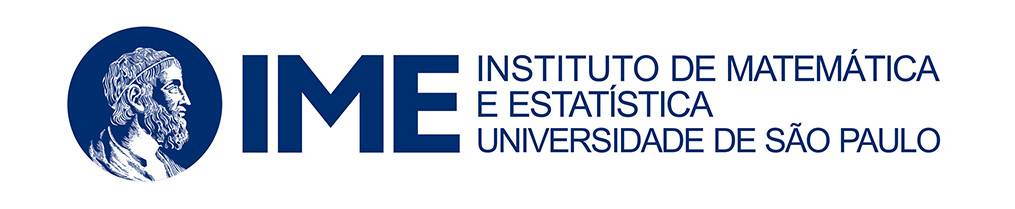
\includegraphics[width=0.6\textwidth]{images/logo_ime.png}\par
	\vspace{2cm}
 
	% {\scshape\LARGE Relatório Científico do projeto na modalidade Bolsa de Iniciação Científica, fomentado pela Fundação de Amparo à Pesquisa do Estado de São Paulo. \par}

	%%%% PROJECT TITLE
	{\huge\bfseries Quantum Walks and its Applications in Quantum Networks  \par}
	\vspace{2cm}

     
\includegraphics[width=0.5\textwidth]{images/umass_logo.png}\par
	\vspace{3cm}
	
	%%%% AUTHOR(S)
	{\Large Scientific report BEPE FAPESP 2023/06452-2 Andre Nogueira Ribeiro}\par
    {\Large Validity period: 08/20/2023 a 12/20/2024}\par
    {\Large Associated period: 08/20/2023 a 02/28/2024}\par
    {\Large Supervisor: Prof. Fabio Kon (IME/USP)}\par
    {\Large Co-supervisor:  Prof. Antonio Jorge Gomes Abelém (UFPA)}\par
    {\Large Supervisor at University of Massachusetts: Prof. Don Towsley(UMass)}\par
	\vspace{1.5cm}
 
\end{titlepage}

\newpage

\tableofcontents

\newpage

\section{Informações gerais do projeto}
    \begin{itemize}
        \item \large Título do Projeto: \\ Computação e Internet Quântica 
    \end{itemize}
    \begin{itemize}
        \item \large Autor: \\
        Andre Nogueira Ribeiro
    \end{itemize}
    \begin{itemize}
        \item \large Instituição sede do projeto: \\
        Instituto de Matemática e Estatística da Universidade de São Paulo
    \end{itemize}
    \begin{itemize}
        \item \large Orientador: \\
        Fabio Kon
    \end{itemize}
    \begin{itemize}
        \item \large Número do projeto de pesquisa:\\
        2022/07594-2 
    \end{itemize}
    \begin{itemize}
        \item \large Período de vigência: \\
        01/08/2022 a 31/07/2023 
    \end{itemize}
    \begin{itemize}
        \item \large Período coberto por este relatório científico: \\
        01/08/2022 a 10/01/2023 
    \end{itemize}
    
    \newpage

\section{Resumo do projeto proposto}
    
    A computação quântica nasceu a partir da ideia de criar uma máquina capaz de simular sistemas quânticos mais complexos, proposta pelo físico Richard Feynman e pelo matemático Yuri Manin. O esforço para tais simulações em computadores clássicos cresce exponencialmente em função do tamanho do sistema, o que as inviabiliza para qualquer problema de tamanho interessante. Além desse foco, estudos na área de algoritmos também obtiveram sucesso com a computação quântica, em que algoritmos consideravelmente mais rápidos do que os clássicos já foram propostos, como o algoritmo de Shor para a fatoração de números.
    
	Destaca-se também, o fato de que a computação quântica é um objeto de estudo com uma gama de novas possibilidades a serem exploradas, o que a torna mais instigante e promissora. No cenário atual, empresas como a Google e a IBM, destaques nesse ramo, possuem máquinas quânticas funcionais, que demonstram a grande relevância desse estudo, ao passo que são capazes de realizar tarefas inacessíveis aos computadores clássicos (conforme publicações da Google em 2019 e da IBM em 2021) . Alguns dos desafios encontrados no trabalho de aprimorar tais computadores são aumentar o número de qubits (unidade básica de memória de um computador quântico), diminuir ruídos e aumentar o tempo de coesão (tempo de duração dos fenômenos quânticos para executar um algoritmo).
 
	Nesta iniciação científica, motivado pelo que foi apresentado, o bolsista, durante o primeiro ano, irá estudar de forma sistemática os principais conceitos da Computação Quântica e da Comunicação Quântica. Em particular, alguns dos  conceitos que serão estudados são qubit, portas lógicas, propriedades da física quântica, circuitos, algoritmos, linguagem de programação em computadores quânticos, interferência, estados de Bell, teleporte quântico, emaranhamento quântico, purificação e correção de erros nesse contexto e repetidores quânticos. Os trabalhos realizados serão disponibilizados publicamente no website do projeto \href{https://interscity.org/quantum-internet/}{https://interscity.org/quantum-internet}.
 
	Por fim, o conhecimento adquirido ao longo desse primeiro ano servirá de base para a proposta a ser desenvolvida no segundo ano do projeto, que envolverá pesquisa original envolvendo a proposição e avaliação de novos protocolos para a Internet Quântica.

\newpage

\section{Resumo das atividades realizadas}
    Nos primeiros seis meses da pesquisa em questão, de título "Computação e Internet Quântica" , compreendeu-se os princípios da computação quântica, como o qubit, as portas lógicas quânticas, alguns algoritmos, as propriedades importantes da física quântica, além das inovações que essa área  pode proporcionar. Após construir essa base teórica e também trabalhar com algo mais prático (circuitos e programação na área quântica), iniciou-se um estudo para compreender os pilares da comunicação quântica.

     O andamento do projeto seguiu o que foi proposto no cronograma descrito no projeto de pesquisa apresentado para a FAPESP sem atrasos. Nenhum assunto foi negligenciado e em acordo com isto, os tópicos estudados durante o semestre foram:
    \begin{enumerate}
        
        \item Princípios da computação quântica
        \item Propriedades da física quântica aplicadas à computação
        \item Algoritmos e circuitos mais complexos
        \item Linguagem de programação voltada para computação quântica (qiskit)
        \item Trabalho com circuitos e programas quânticos
        \item Princípios da comunicação quântica
    \end{enumerate}
    
    Apresentarei em seguida o que foi estudado em cada tópico. Vale ressaltar que o projeto utiliza o site \href{https://interscity.org/quantum-internet/}{https://interscity.org/quantum-internet/} para disponibilizar alguns conteúdos estudados.


\newpage

\section{Realizações do período}
    Nesta seção mostrarei com mais detalhes cada uma das atividades realizadas, de modo a resumir os conteúdos abordados e a transmitir os resultados dos estudos referentes à pesquisa.
    
    \subsection{Princípios da computação quântica}
    Nesta seção abordarei os conceitos que estudei pertencentes à base da computação quântica. A partir dos conceitos estudados nessa seção preparei slides iniciais que foram apresentados para o orientador Fabio Kon. Essa apresentação, mais para frente, foi revisada e aprimorada com novos conteúdos gerando uma nova apresentação disponibilizada na  \href{https://interscity.org/quantum-internet/}{página do projeto}. Além disso, modifiquei o mesmo conteúdo dessa apresentação para a língua norte americana e apresentei esse novo trabalho para o grupo de sistemas IME-USP.

        \subsubsection{Relevâncias da computação quântica}
        Dentre os principais aspectos presentes nesse tópico, tem-se a computação quântica permite melhorar a simulação de sistemas quânticos, haja vista que, em computadores clássicos, ela cresce exponencialmente em função do tamanho do sistema enquanto em computadores quânticos não. Além disso, existem problemas em que algoritmos quânticos apresentam diminuição significativa no gasto de memória e de velocidade o que tem extrema relevância dado que a atualidade é cercada por aplicações de softwares e consequentemente algoritmos. Por fim, as propriedades dos dispositivos quânticos possivelmente permitem grandes melhoras associadas à área de segurança digital. 

        \subsubsection{Qubit}
        O qubit é a unidade básica de memória de um computador quântico e possui mais de dois estados além dos clássicos 0 ou 1. Devido às propriedades quânticas, o qubit admite a coexistência do 0 e 1,o que pode ocorrer de infinitas formas distintas. Apesar de ter infinitos estados diferentes, isso só ocorre antes de uma medição. Ao realizar uma verificação do estado do qubit a resposta é 0 ou é 1, ou seja, quando o qubit é medido ele "vira" (colapsa é o termo mais utilizado) 0 ou 1. É possível utilizar desses infinitos estados sem verificá-los, o que reflete em um ganho computacional.
    
        \subsubsection{Modelo Matemático}
        Por meio das referências bibliográficas e com foco no capítulo 2.1 do livro "Quantum Computation and Quantum Information", que faz uma revisão da algebra linear necessária para entender o modelo matemático aplicado à computação quântica, estudei a teoria por trás da representação de um sistema de computação quântica. O qubit, a unidade básica de memória do computador quântico pode ser representada por um vetor bidimensional e as portas lógicas que atuam nesse qubit por matrizes unitárias. 

        O estado de um qubit é da forma $ v = a\ket{0} + b\ket{1}$, sendo que $\ket{0}$ é o vetor (1,0), que corresponde ao estado com probabilidade 1 de colapsar em 0, e $\ket{1}$ é o vetor (0,1), que representa o estado com probabilidade 1 de colapsar em 1. Tem-se que $|a|$ ao quadrado é a probabilidade desse qubit ser 0 após a medição e $|b|$ ao quadrado é a probabilidade dele ser 1. Naturalmente, para funcionar, $|a|$ ao quadrado somado com$|b|$ ao quadrado é igual a 1.
    
        Vale ressaltar que, muitas vezes, trabalha-se com o estado de vários qubits juntos e isso é representado por um vetor de mais dimensões. A cada qubit a mais dobra-se o número de dimensões. Um estado dado por 2 qubits é representado por um vetor de 4 dimensões por exemplo.
        
        Existe também uma representação comum que associa o qubit a uma esfera, denominada esfera de Bloch, ou seja, um vetor 3d, que possui também a fase global do qubit(uma propriedade física associada a ele). Nessa seção também foi necessário entender as relações  probabilísticas presentes nesse contexto.
    
        \subsubsection{Portas lógicas}
        Em um circuito, a porta lógica é responsável por alterar de algum modo específico a informação que passa por ela. No contexto quântico, elas são representadas por matrizes quadradas unitárias(uma porta que atua em um qubit é uma matriz unitária 2x2 enquanto uma porta lógica que atua em dois qubits é uma matriz unitária 4x4).
    
        Alguma das portas lógicas quânticas estudadas foram a Porta de Hadamard, que realiza uma superposição de estados com igual probabilidade, a porta X, que inverte as probabilidades de se medir 0 e 1 em um qubit e a porta CNOT, que atua em dois qubits com um mecanismo que, dependendo do estado de um deles(chamado qubit de controle), atua ou não no outro(qubit alvo). Outras portas também estudadas foram a porta Toffoli, a porta de Fase e a porta T.
    
        Na apresentação está a representação matricial de algumas dessas portas. O estudo delas foi essencial para futuramente entender circuitos quânticos mais complexos.
    
        \subsubsection{Desafios}
        Os principais pontos nesse tópico, que foram explicitados na apresentação, são a dificuldade em manter efeitos quânticos ao passo que o experimento deixa de ser algo microscópico e a necessidade de que o ambiente permita efeitos quânticos por um tempo maior que um segundo, que é algo razoável para rodar certos algoritmos(esse tempo é denominado tempo de coesão). Por fim, sabe-se que um computador clássico consegue simular um computador quântico com 56 qubits, portanto, o computador quântico, para ser relevante, deve possuir mais do que 56 qubits.

        Percebe-se que a dificuldade na área da computação quântica reside tanto em fatores físicos quanto na dificuldade de superar as tecnologias clássicas desenvolvidas nas últimas décadas.  

    \subsection{Propriedades da física quântica aplicadas à computação}
        Nesta seção abordarei o que foi feito para estudar algumas partes mais teóricas que se relacionam com a computação quântica além de expor dois conceitos importantes.
        
        \subsubsection{Leitura}
        Para esse tópico realizei a leitura dos capítulos 2.2.1-State space, 2.2.2-Evolution, 2.2.3-Quantum measurement, 2.2.4-Distinguishing quantum states, 2.2.5-Projective measurements, 2.2.6-POVM measurements e o 2.2.7-Phase, do livro Quantum Computation and Quantum Information Michael A.Nielsen Isaac L. Chuang,10th Anniversary Edition. 
        
        Isso foi feito de modo a compreender melhor alguns aspectos teóricos físicos e matemáticos utilizados na construção da computação quântica. Nessa parte do livro, foi necessária uma leitura cuidadosa e acompanhada de pesquisas constantes devido a notação matemática rebuscada, principalmente na parte de álgebra linear.
        
        \subsubsection{Superposição e Entrelaçamento quântico}
        Julguei que os conceitos de superposição e entrelaçamento quântico são notáveis na área e por isso estudei um pouco mais profundamente sobre eles.
    
        De maneira resumida, a superposição consiste no fato de que um sistema quântico pode assumir todos os estados possíveis simultaneamente. No caso da computação, o estado do qubit é uma superposição do 0 e do 1, ou seja, ele é 0 e 1 ao mesmo tempo. 
    
        O conceito de entrelaçamento quântico sugere uma relação entre duas partículas que independe da distância entre elas. No caso da computação, se temos dois qubits entrelaçados quando um é medido o outro colapsará para o mesmo estado que foi medido no outro.

    \subsection{Algoritmos e circuitos mais complexos}
        Nesta seção demostrarei o estudo realizado sobre dois importantes algoritmos na área da computação quântica, o algoritmo de Shor e o algoritmo de Grover.
        
        \subsubsection{Algoritmo de Shor}
        Esse algoritmo é um dos algoritmos mais famosos da computação quântica pois é utilizado na fatoração de números. Nesse contexto, o algoritmo clássico mais eficiente consome tempo exponencial enquanto o algoritmo quântico faz essa tarefa em tempo polinomial. Essa expressiva melhora com o algoritmo de Shor representa um grande evento associado à segurança digital, que em muitos casos é baseada na fatoração da multiplicação de grandes números primos.
        
        Uma referência importante neste estudo, que complementou e aprimorou o estudo sobre o algoritmo de Shor, foi a parte referente a esse algoritmo da "Qiskit Global Summer School 2020". São 6 vídeos densos de aproximadamente 50 minutos cada disponibilizados no canal qiskit do youtube.
        
        Com o conhecimento adquirido, fiz uma apresentação sobre o algoritmo de Shor, que foi realizada para o grupo de pesquisa que contém o orientador e o coorientador do projeto. Vale ressaltar que os slides que explicam melhor o conteúdo estudado estão disponíveis no site \href{https://interscity.org/quantum-internet/}{página do projeto}.
    
        \subsubsection{Algoritmo de Grover}
    
        Esse algoritmo faz uma busca em uma lista de n elementos com um consumo de tempo proporcional a raiz de n enquanto o algoritmo clássico consome tempo proporcional a n. Exemplificando, para uma entrada de tamanho $10^{6}$ o algoritmo quântico é $10^{3}$ vezes mais rápido desconsiderando as constantes envolvidas. Sua lógica é baseada principalmente na inversão da fase de um estado considerado provavelmente bom(que provavelmente seja a resposta). O objetivo é aumentar a probabilidade(amplitude) desses estados para que ao final, o estado observado seja associado à resposta correta.

    \subsection{Linguagem de programação voltada para computação quântica (qiskit)}
        Instalei e testei a linguagem qiskit, além de fazer alguns programas. Serão apresentados três deles sendo que cada um foi executado mais de uma vez com pequenas modificações com intuito de haver familiarização e fazer testes utilizando a linguagem. Os três programas mencionados nesta seção estão na \href{https://interscity.org/quantum-internet/}{página do projeto} em ordem.
    
        \subsubsection{Dois programas introdutórios}
        
        O Primeiro programa testa algumas funcionalidades básicas como verificar a versão do qiskit, aplicação de portas lógicas e conectar com a conta IBM. Em seguida, as células constroem um circuito quântico que faz uma aplicação de uma porta de Hadamard no primeiro qubit e em seguida aplica uma uma porta CNOT. Isso cria uma superposição de dois estados, com 50\% de chance da saída colapsar em 00 e 50\% de chance da saída colapsar em 11, o que pode ser observado no histograma que representa a quantidade de vezes que a saída colapsou em cada estado. 
        
        Após isso, o programa constrói o mesmo circuito anterior porém agora a execução do circuito é feita em um computador quântico real a partir da conexão com a conta pessoal na IBM. O resultado não é preciso como na simulação pois o computador quântico real apresenta erros. 
    
        O segundo programa é uma continuação da introdução a linguagem qiskit, demonstrando algumas formas de visualização dos circuitos e das portas lógicas.
        
        \subsubsection{Protocolo de teletransporte de informação}    
    
        O terceiro programa constrói um protocolo que teletransporta o estado do qubit 0 para o qubit 2. O protocolo inicia-se após a primeira barreira(isso esta no notebook presente na página do projeto). Nesse ponto, o qubit 0 possui um estado com 100\% de chance de colapsar em 1 e esse estado é transmitido para o qubit 2. Isso pode ser observado no histograma em que todos os estados possíveis contém o qubit 2 colapsado em 1.

        Vale ressaltar que os histogramas presentes nos notebooks mostram quantas vezes a resposta foi uma dada sequência de qubits. Por exemplo, se a barra do histograma que corresponde a saída "01" apresentar altura 521 e a barra do "10" ter altura 503, isso significa que o programa foi rodado 1024 vezes, sendo que em 521 delas a resposta obtida foi 0 para o segundo qubit e 1 para o primeiro e em 503 a resposta foi a outra. Percebe-se que a ordem da resposta no histograma é invertida, ou seja, o primeiro valor corresponde ao último qubit.

    \subsection{Trabalho com circuitos e programas quânticos}

        \subsubsection{Implementação}
        Implementei dois algoritmos conhecidos, o algoritmo de Bernstein-Vazirani e o algoritmo de Shor. Ambos estão na \href{https://interscity.org/quantum-internet/}{página do projeto} (dois ultimos algoritmos). 
    
        Como o algoritmo de Shor já foi mencionado falarei apenas do algoritmo de Bernstein-Vazirani. Esse algoritmo está associado a uma função f(x) = (s . x)mod 2 e serve para acertar uma palavra secreta de k dígitos binários com apenas uma chamada da função. Esse algoritmo é uma demostração relativamente simples de um programa quântico que apresenta ganho no custo computacional quando comparado a um algoritmo clássico, que nesse caso iria chamar k vezes a função. Vale ressaltar que o programa foi feito de maneira genérica podendo-se colocar qualquer palavra secreta binária na variável "secreta".

        \subsubsection{Estudo}
            Estudei mais dois algoritmos, o algoritmo de Deutsch-Jozsa algorithm eo algoritmo de Simon.
            \\
           
            O algoritmo de Deutsch-Jozsa foi o primeiro algoritmo quântico que apresentou melhora em relação a complexidade quando comparado com um algoritmo clássico. 
            
            Para ele é dada uma função que recebe uma string de bits e retorna 0 ou 1. A promessa é que essa função é constante(0 ou 1 para todas as entradas) ou balanceada(0 para metade dos inputs e 1 para a outra metade) e o objetivo é descobrir em qual dessas classes a função se encaixa.
            
            No caso clássico deve-se chamar a função pelo menos metade dos inputs mais um, ou seja 2 elevado a (n-1) mais uma vezes, ao passo que um string de n bits possibilita 2 elevado a n entradas. Já para o caso quântico resolve-se o problema com apenas uma chamada da função e utiliza-se de que a função balanceada não altera a fase global do estado nos qubits de entrada.
        
            O circuito referente a esse algoritmo é:
        
            \begin{figure}[h]
            \begin{center}
            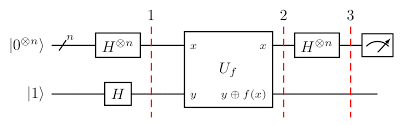
\includegraphics[width=13cm]{images/dj.png}
            \end{center}
            \end{figure}

            \newpage
            
            O algoritmo de Simon consiste em descobrir se uma dada função é 1 para 1 ou 2 para 1 em um cenário que apresenta apenas essas duas possibilidades. Uma função 1 pra 1 significa que um elemento da imagem apresenta apenas um correspondente no domínio enquanto a função 2 pra 1 significa que um elemento da imagem possui dois correspondentes no domínio.
            
            Esse problema foi o primeiro problema quântico em que verificou-se uma solução exponencialmente melhor para um computador quântico em relação ao clássico. A solução quântica é linear enquanto a solução quântica é exponencial.
            
            As principais referências nesse estudo foram o site qiskit.org e o canal do youtube ArturEkert.
        
            O circuito referente a esse algoritmo é:
        
            \begin{figure}[h]
            \begin{center}
            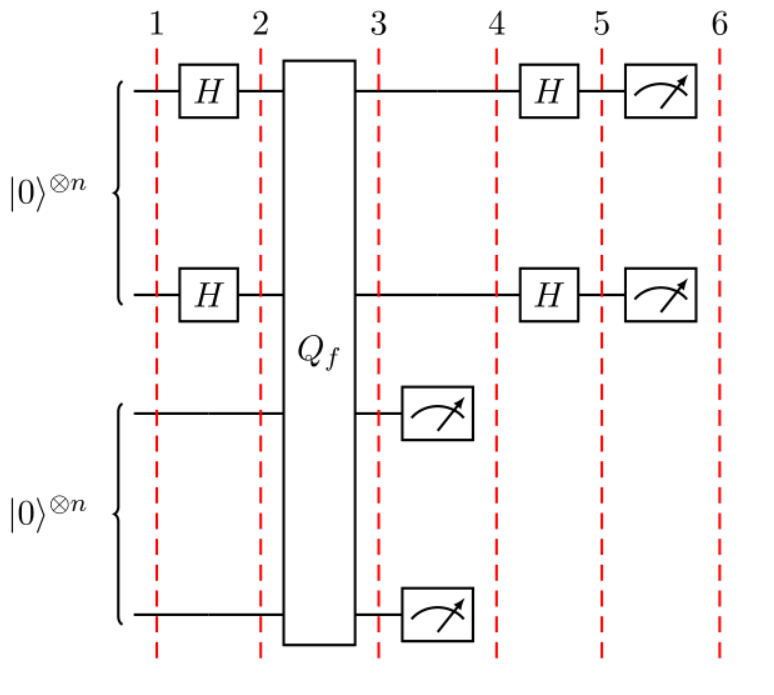
\includegraphics[width=10cm]{images/simons.png}
            \end{center}
            \end{figure}

    \subsection{Princípios da comunicação quântica}
    
        Estudei esse tema por meio do artigo "Quantum internet: A vision for the road ahead-Stephanie Wehner, David Elkouss, Ronald Hanson" e também pelo material associado à comunicação quântica do XXXVIII Simpósio Brasileiro de Redes de Computadores e Sistemas Distribuídos, produzido pelo professor Antônio Jorge Abelém. 
        
        Primeiramente, a intenção de estudar e tornar realidade uma internet quântica sugere criar novas tecnologias a partir da possibilidade de comunicação quântica entre quaisquer dois pontos do planeta. Nesse ramo, aplicações importantes já foram identificadas, incluindo segurança na comunicação, sincronização do "clock", identificação segura de um usuário, economia exponencial em comunicação e também acesso seguro a computadores quânticos remotos na nuvem.
        
        Uma internet quântica consiste em três elementos básicos de hardware quântico. Primeiro precisa-se de uma conexão física que suporte a transmissão de qubits. Em segundo lugar, precisa-se de um meio para conseguir aumentar as distâncias de transmissão e isso é feito através de repetidores quânticos. Por fim, necessita-se de processadores quânticos conectados à internet quântica para processar a informação recebida. Vale ressaltar que, segundo o artigo em questão, uma internet quântica pretende complementar a comunicação clássica e não substituí-la.

    \subsection{Outras atividades realizadas}
        Nesta seção serão descritas outras atividades realizadas durante o período de pesquisa para complementar o estudo.

        Primeiramente, vale ressaltar que os primeiros vídeos da "qiskit global summer school 2020" e o site \href{https://qiskit.org}{https://qiskit.org} serviram para revisar e aprofundar os conhecimentos acerca das bases da computação quântica. Por mais que esta não fosse uma referência presente no projeto de pesquisa, devido a qualidade dos vídeos e textos, julgou-se pertinente utilizar este conteúdo. 

        Outro meio que complementou os estudos foram as duas defesas de mestrado de alunos do IME-USP que assiste, ambas sobre computação quântica passando pelos temas mostrados nesse relatório entre outros, como jogos de comunicação. Isso foi realizado de modo a compreender as apresentações dos mestrandos, além de solidificar o conhecimento na área e entender como uma apresentação de mestrado funciona.

        Também assisti 3 apresentações do aluno de mestrado orientado pelo professor Antônio Jorge Abelém(coorientador do projeto). A primeira apresentação foi sobre as bases da computação quântica, a segunda foi uma demonstração de como rodar programas quânticos em computadores quânticos pelo site da IBM e a terceira foi uma introdução à comunicação quântica.
    
        Por fim, durante o projeto acompanhei e li algumas notícias que se encaixavam no contexto da pesquisa. Alguns dos temas foram \href{https://www.nature.com/articles/s41586-019-1666-5}{supremacia quântica}, \href{https://beta.nsf.gov/news/tiny-optical-cavities-could-make-quantum-networks-possible}{descobertas na área de comunicação quântica}, \href{https://beta.nsf.gov/news/toward-unhackable-quantum-internet}{segurança no contexto da computação quântica} e \href{https://www.nytimes.com/2022/10/04/science/nobel-prize-physics-winner.html?unlocked_article_code=AAAAAAAAAAAAAAAACEIPuonUktbfqYhlSFUbBybOVtkqqBaLwv7IyrE4w2fkLTqYDC5C3v8UCJPF5EbLY6d5Idsv2jDRDPlwDIgSft0ghOlOIx4qDACyvpqPnJlCLXhv9d3iAG1z0ZmTAfVlqjHnKzjgdLk6zeLk5x7dPmO9D6TYwmRhcFg-2eZtcV-g3HUPxqfXQKUiipQlg6BXVt0tTiwAZSKKo_HqFxx4Xd2GZRne4QAzMPpLDXCRxZXPruJdL3gBTA7OX3h94m0j6NpDONJxPK33LxcoecuWkqwcm8vTEA3ohQWqE9s2-L6Y&smid=nytcore-ios-share&referringSource=articleShare}{prêmios da área}.
    
\newpage

% \section{Descrição e avaliação do Apoio Institucional recebido no período}
%     O Departamento de Ciência da Computação do IME-USP ofereceu ao aluno todo apoio necessário mesmo mediante a pandemia viral de Covid-19. O aluno contou com uma ótima infraestrutura para realizar seus estudos incluindo serviços de computação e acesso a periódicos. Por fim, os professores do departamento foram sempre muito solícitos em tirar dúvidas e debater tópicos do projeto, em especial os orientadores do mesmo, que 

% \newpage

\section{Plano de atividades para o próximo período}
    Nestes seis primeiros meses estudei os princípios da computação quântica, passando pelos principais pilares da área tanto teóricos quanto alguns mais práticos(implementação de programas). Foi iniciado também o estudo na parte de comunicação e internet quântica.

     Em acordo com o que foi proposto no projeto de pesquisa, o intuito é, com ajuda dos conhecimentos adquiridos até agora, direcionar os próximos trabalhos para a área da comunicação e Internet quântica. O início da pesquisa será baseado nas bases conceituais da área e em seguida tem-se o objetivo de propor uma linha autoral de pesquisa original em Internet Quântica.

     Na área da comunicação quântica, uma Internet quântica permitirá aplicações que extrapolam o escopo da Internet clássica, principalmente no âmbito da segurança, devido às propriedades da física quântica, que permitem proteger os dados durante a troca de informações e também compartilhar estados quânticos entrelaçados entre duas ou mais partes. No entanto, os sinais quânticos são muito frágeis e não podem ser amplificados ou copiados, pois, para se copiar um qubit, precisaria medi-lo, o que o faria colapsar, inviabilizando o processo desejado. Desafios como este criam uma gama de possibilidades de estudos para resolvê-los e, por conseguinte, ampliam a relevância das pesquisas na área.

     Dado isso, pretende-se dar continuidade ao cronograma presente no projeto de pesquisa. Os próximos tópicos a serem estudados são inovações recentes na área da comunicação quântica e internet quântica, além de complementar os estudos sobre os princípios da comunicação quântica e continuar alimentando a página do projeto e apresentando seminários. Como mencionado anteriormente, deseja-se nesse período elaborar uma proposta de pesquisa autoral e original sobre o tema protocolos de roteamento para Internet Quântica. 

\subsection{Cronograma}
Para exemplificar melhor, segue o cronograma:

\begin{table}[h]
\begin{tabular}{|l|l|l|l|l|l|l|}
\hline
\begin{tabular}[c]{@{}l@{}}meses\\ ----------\\ tópicos\end{tabular}                                                                              & 7 & 8 & 9 & 10 & 11 & 12 \\ \hline
Princípios da comunicação quântica                                                                                                                & X &   &   &    &    &    \\ \hline
Estudos recentes na área da comunicação quântica                                                                                                  & X & X &   &    &    &    \\ \hline
Internet Quântica                                                                                                                                 &   & X & X & X  & X  & X  \\ \hline
\begin{tabular}[c]{@{}l@{}}Elaborar uma proposta autoral de pesquisa sobre \\ o tema protocolos de roteamento para Internet Quântica\end{tabular} &   &   &   & X  & X  & X  \\ \hline
\begin{tabular}[c]{@{}l@{}}Apresentação de seminários para o grupo de \\ pesquisa sobre os assuntos estudados\end{tabular}                        & X & X & X & X  & X  & X  \\ \hline
Disponibilização do conteúdo estudado no site do projeto                                                                                          & X & X & X & X  & X  & X  \\ \hline
\end{tabular}
\end{table}

 Serão utilizadas as referências que foram descritas no projeto de pesquisa para tais temas. Vale ressaltar que também pretendemos solicitar uma bolsa de estágio de pesquisa no exterior(BEPE) no próximo semestre.
     

\newpage

\section{Referências Bibliográficas}
    Além de algumas referências citadas durante o relatório em questão o material estudado foi:\\
    
    [Abelem et al. 2020] - Abelém, A. J. G. ; Vardoyan, Gayane ; Towsley, Don . Quantum Internet: The Future of Internetworking. In: Minicursos do XXXVIII Simpósio Brasileiro de Redes de Computadores e Sistemas Distribuídos. 1ed.: SBC, 2020, p. 48-90. doi.org/10.5753/sbc.5033.7.2.\\
    
    [Arute et al. 2019]-Arute, F., Arya, K., Babbush, R. et al. Quantum supremacy using a programmable superconducting processor. Nature 574, 505–510 (2019). doi.org/10.1038/s41586-019-1666-5.\\
    
    [Courtland 2017]-Courtland, R. ‘‘Google aims for quantum computing supremacy; News,’’ IEEE Spectr., vol. 54, no. 6, pp. 9–10, Jun. 2017.\\
    
    [Nielsen 2010] - Nielsen, Michael A., C. I. (2010).Quantum computation and quantum information:  10th Anniversary Edition.  Cambridge University Press, New York, NY,USA.\\
    
    [Portugal et al. 2012] - Uma Introdução à Computação Quântica- Portugal, Renato; Lavor, Carlile Campos; Carvalho, Luiz Mariano; Maculan, Nelson.\\
    
    [Portugal et al. 2019] - Jornada de Atualização em Informática 2019, SBC(Sociedade Brasileira de Computação), capítulo 1, Introdução à Programação de Computadores Quânticos-Renato Portugal, Franklin Marquezino.\\

    [Wehner et al. 2018]- Wehner, Stephanie, Elkouss, D., and Hanson, R. “Quantum internet: A vision for the road ahead.” Science, 362(1):303, 2018.\\


\newpage

\section{Informações gerais do projeto}
    \begin{itemize}
        \item \large Título do Projeto: \\ Computação e Internet Quântica 
    \end{itemize}
    \begin{itemize}
        \item \large Autor: \\
        Andre Nogueira Ribeiro
    \end{itemize}
    \begin{itemize}
        \item \large Instituição sede do projeto: \\
        Instituto de Matemática e Estatística da Universidade de São Paulo
    \end{itemize}
    \begin{itemize}
        \item \large Orientador: \\
        Fabio Kon
    \end{itemize}
    \begin{itemize}
        \item \large Número do projeto de pesquisa:\\
        2022/07594-2 
    \end{itemize}
    \begin{itemize}
        \item \large Período de vigência: \\
        01/08/2022 a 31/07/2023 
    \end{itemize}
    \begin{itemize}
        \item \large Período coberto por este relatório científico: \\
        01/08/2022 a 05/05/2023 
    \end{itemize}
    
    \newpage

\section{Resumo do projeto proposto}
    
    A computação quântica nasceu a partir da ideia de criar uma máquina capaz de simular sistemas quânticos mais complexos, proposta pelo físico Richard Feynman e pelo matemático Yuri Manin. O esforço para tais simulações em computadores clássicos cresce exponencialmente em função do tamanho do sistema, o que as inviabiliza para qualquer problema de tamanho interessante. Além desse foco, estudos na área de algoritmos também obtiveram sucesso com a computação quântica, em que algoritmos consideravelmente mais rápidos do que os clássicos já foram propostos, como o algoritmo de Shor para a fatoração de números.
    
	Destaca-se também, o fato de que a computação quântica é um objeto de estudo com uma gama de novas possibilidades a serem exploradas, o que a torna mais instigante e promissora. No cenário atual, empresas como a Google e a IBM, destaques nesse ramo, possuem máquinas quânticas funcionais, que demonstram a grande relevância desse estudo, ao passo que são capazes de realizar tarefas inacessíveis aos computadores clássicos (conforme publicações da Google em 2019 e da IBM em 2021) . Alguns dos desafios encontrados no trabalho de aprimorar tais computadores são aumentar o número de qubits (unidade básica de memória de um computador quântico), diminuir ruídos e aumentar o tempo de coesão (tempo de duração dos fenômenos quânticos para executar um algoritmo).
 
	Nesta iniciação científica, motivado pelo que foi apresentado, o bolsista, durante o primeiro ano, irá estudar de forma sistemática os principais conceitos da Computação Quântica e da Comunicação Quântica. Em particular, alguns dos  conceitos que serão estudados são qubit, portas lógicas, propriedades da física quântica, circuitos, algoritmos, linguagem de programação em computadores quânticos, interferência, estados de Bell, teleporte quântico, emaranhamento quântico, purificação e correção de erros nesse contexto e repetidores quânticos. Os trabalhos realizados serão disponibilizados publicamente no website do projeto \href{https://interscity.org/quantum-internet/}{https://interscity.org/quantum-internet}.
 
	Por fim, o conhecimento adquirido ao longo desse primeiro ano servirá de base para a proposta a ser desenvolvida no segundo ano do projeto, que envolverá pesquisa original envolvendo a proposição e avaliação de novos protocolos para a Internet Quântica.

\newpage

\section{Resumo das atividades realizadas}
    Desde o início até o momento atual da pesquisa em questão, de título ``Computação e Internet Quântica'' , compreendeu-se os princípios da computação quântica, como o qubit, as portas lógicas quânticas, alguns algoritmos, as propriedades importantes da física quântica, além das inovações que essa área  pode proporcionar. Após construir essa base teórica e também trabalhar com algo mais prático (circuitos e programação na área quântica), o aluno direcionou os estudos para a área de comunicação e Internet quântica.

     O andamento do projeto seguiu o que foi proposto no cronograma descrito no projeto de pesquisa apresentado para a FAPESP sem atrasos. Nenhum assunto foi negligenciado e em acordo com isto, os tópicos estudados durante o período foram:
    \begin{enumerate}
        
        \item Princípios da computação quântica
        \item Propriedades da física quântica aplicadas à computação
        \item Algoritmos e circuitos mais complexos
        \item Linguagem de programação voltada para computação quântica (qiskit)
        \item Trabalho com circuitos e programas quânticos
        \item Comunicação quântica
        \item Internet quântica
    \end{enumerate}
    
    Apresentarei em seguida o que foi estudado em cada tópico. Vale ressaltar que o projeto utiliza o site \href{https://interscity.org/quantum-internet/}{https://interscity.org/quantum-internet/} para disponibilizar alguns conteúdos estudados.
 
\newpage

\section{Realizações do período}
    Nesta seção mostrarei com mais detalhes cada uma das atividades realizadas, de modo a resumir os conteúdos abordados e a transmitir os resultados dos estudos referentes à pesquisa.
    
    \subsection{Princípios da computação quântica}
    Nesta seção abordarei os conceitos que estudei pertencentes à base da computação quântica. A partir dos conceitos estudados nessa seção preparei slides iniciais que foram apresentados para o orientador Fabio Kon. Essa apresentação, mais para frente, foi revisada e aprimorada com novos conteúdos gerando uma nova apresentação disponibilizada na  \href{https://interscity.org/quantum-internet/}{página do projeto}. Além disso, modifiquei o mesmo conteúdo dessa apresentação para a língua norte americana e apresentei esse novo trabalho para o grupo de sistemas IME-USP.

        \paragraph{Relevâncias da computação quântica.}
        Dentre os principais aspectos presentes nesse tópico, tem-se a computação quântica permite melhorar a simulação de sistemas quânticos, haja vista que, em computadores clássicos, ela cresce exponencialmente em função do tamanho do sistema enquanto em computadores quânticos não. Além disso, existem problemas em que algoritmos quânticos apresentam diminuição significativa no gasto de memória e de velocidade o que tem extrema relevância dado que a atualidade é cercada por aplicações de softwares e consequentemente algoritmos. Por fim, as propriedades dos dispositivos quânticos possivelmente permitem grandes melhoras associadas à área de segurança digital. 

        \paragraph{Qubit.}
        O qubit é a unidade básica de memória de um computador quântico e possui mais de dois estados além dos clássicos 0 ou 1. Devido às propriedades quânticas, o qubit admite a coexistência do 0 e 1,o que pode ocorrer de infinitas formas distintas. Apesar de ter infinitos estados diferentes, isso só ocorre antes de uma medição. Ao realizar uma verificação do estado do qubit a resposta é 0 ou é 1, ou seja, quando o qubit é medido ele ``vira''  (colapsa é o termo mais utilizado) 0 ou 1. É possível utilizar desses infinitos estados sem verificá-los, o que reflete em um ganho computacional.
    
        \paragraph{Modelo Matemático.}
        Por meio das referências bibliográficas e com foco no capítulo 2.1 do livro ``Quantum Computation and Quantum Information'', que faz uma revisão da algebra linear necessária para entender o modelo matemático aplicado à computação quântica, estudei a teoria por trás da representação de um sistema de computação quântica. O qubit, a unidade básica de memória do computador quântico pode ser representada por um vetor bidimensional e as portas lógicas que atuam nesse qubit por matrizes unitárias. 

        O estado de um qubit é da forma $ v = a\ket{0} + b\ket{1}$, sendo que $\ket{0}$ é o vetor (1,0), que corresponde ao estado com probabilidade 1 de colapsar em 0, e $\ket{1}$ é o vetor (0,1), que representa o estado com probabilidade 1 de colapsar em 1. Tem-se que $|a|$ ao quadrado é a probabilidade desse qubit ser 0 após a medição e $|b|$ ao quadrado é a probabilidade dele ser 1. Naturalmente, para funcionar, $|a|$ ao quadrado somado com$|b|$ ao quadrado é igual a 1.
    
        Vale ressaltar que, muitas vezes, trabalha-se com o estado de vários qubits juntos e isso é representado por um vetor de mais dimensões. A cada qubit a mais dobra-se o número de dimensões. Um estado dado por 2 qubits é representado por um vetor de 4 dimensões por exemplo.
        
        Existe também uma representação comum que associa o qubit a uma esfera, denominada esfera de Bloch, ou seja, um vetor 3d, que possui também a fase global do qubit (uma propriedade física associada a ele). Nessa seção também foi necessário entender as relações  probabilísticas presentes nesse contexto.
    
        \paragraph{Portas lógicas.}
        Em um circuito, a porta lógica é responsável por alterar de algum modo específico a informação que passa por ela. No contexto quântico, elas são representadas por matrizes quadradas unitárias (uma porta que atua em um qubit é uma matriz unitária 2x2 enquanto uma porta lógica que atua em dois qubits é uma matriz unitária 4x4).
    
        Alguma das portas lógicas quânticas estudadas foram a Porta de Hadamard, que realiza uma superposição de estados com igual probabilidade, a porta X, que inverte as probabilidades de se medir 0 e 1 em um qubit e a porta CNOT, que atua em dois qubits com um mecanismo que, dependendo do estado de um deles (chamado qubit de controle), atua ou não no outro (qubit alvo). Outras portas também estudadas foram a porta Toffoli, a porta de Fase e a porta T.
    
        Na apresentação está a representação matricial de algumas dessas portas. O estudo delas foi essencial para futuramente entender circuitos quânticos mais complexos.
    
        \paragraph{Desafios.}
        Os principais pontos nesse tópico, que foram explicitados na apresentação, são a dificuldade em manter efeitos quânticos ao passo que o experimento deixa de ser algo microscópico e a necessidade de que o ambiente permita efeitos quânticos por um tempo maior que um segundo, que é algo razoável para rodar certos algoritmos (esse tempo é denominado tempo de coesão). Por fim, sabe-se que um computador clássico consegue simular um computador quântico com 56 qubits, portanto, o computador quântico, para ser relevante, deve possuir mais do que 56 qubits.

        Percebe-se que a dificuldade na área da computação quântica reside tanto em fatores físicos quanto na dificuldade de superar as tecnologias clássicas desenvolvidas nas últimas décadas.  

    \subsection{Propriedades da física quântica aplicadas à computação}
        Nesta seção abordarei o que foi feito para estudar algumas partes mais teóricas que se relacionam com a computação quântica além de expor dois conceitos importantes.
        
        \paragraph{Leitura.}
        Para esse tópico realizei a leitura dos capítulos 2.2.1-State space, 2.2.2-Evolution, 2.2.3-Quantum measurement, 2.2.4-Distinguishing quantum states, 2.2.5-Projective measurements, 2.2.6-POVM measurements e o 2.2.7-Phase, do livro ``Quantum Computation and Quantum Information Michael A.Nielsen Isaac L. Chuang,10th Anniversary Edition''. 
        
        Isso foi feito de modo a compreender melhor alguns aspectos teóricos físicos e matemáticos utilizados na construção da computação quântica. Nessa parte do livro, foi necessária uma leitura cuidadosa e acompanhada de pesquisas constantes devido a notação matemática rebuscada, principalmente na parte de álgebra linear.
        
        \paragraph{Superposição e Entrelaçamento quântico.}
        Julguei que os conceitos de superposição e entrelaçamento quântico são notáveis na área e por isso estudei um pouco mais profundamente sobre eles.
    
        De maneira resumida, a superposição consiste no fato de que um sistema quântico pode assumir todos os estados possíveis simultaneamente. No caso da computação, o estado do qubit é uma superposição do 0 e do 1, ou seja, ele é 0 e 1 ao mesmo tempo. 
    
        O conceito de entrelaçamento quântico sugere uma relação entre duas partículas que independe da distância entre elas. No caso da computação, se temos dois qubits entrelaçados quando um é medido o outro colapsará para o mesmo estado que foi medido no outro.

    \subsection{Algoritmos e circuitos mais complexos}
        Nesta seção demostrarei o estudo realizado sobre dois importantes algoritmos na área da computação quântica, o algoritmo de Shor e o algoritmo de Grover.
        
        \paragraph{Algoritmo de Shor.}
        Esse algoritmo é um dos algoritmos mais famosos da computação quântica pois é utilizado na fatoração de números. Nesse contexto, o algoritmo clássico mais eficiente consome tempo exponencial enquanto o algoritmo quântico faz essa tarefa em tempo polinomial. Essa expressiva melhora com o algoritmo de Shor representa um grande evento associado à segurança digital, que em muitos casos é baseada na fatoração da multiplicação de grandes números primos.
        
        Uma referência importante neste estudo, que complementou e aprimorou o estudo sobre o algoritmo de Shor, foi a parte referente a esse algoritmo da ``Qiskit Global Summer School 2020''. São 6 vídeos densos de aproximadamente 50 minutos cada disponibilizados no canal qiskit do youtube.
        
        Com o conhecimento adquirido, fiz uma apresentação sobre o algoritmo de Shor, que foi realizada para o grupo de pesquisa que contém o orientador e o coorientador do projeto. Vale ressaltar que os slides que explicam melhor o conteúdo estudado estão disponíveis no site \href{https://interscity.org/quantum-internet/}{página do projeto}.
    
        \paragraph{Algoritmo de Grover.}
        Esse algoritmo faz uma busca em uma lista de n elementos com um consumo de tempo proporcional a raiz de n enquanto o algoritmo clássico consome tempo proporcional a n. Exemplificando, para uma entrada de tamanho $10^{6}$ o algoritmo quântico é $10^{3}$ vezes mais rápido desconsiderando as constantes envolvidas. Sua lógica é baseada principalmente na inversão da fase de um estado considerado provavelmente bom (que provavelmente seja a resposta). O objetivo é aumentar a probabilidade (amplitude) desses estados para que ao final, o estado observado seja associado à resposta correta.

    \subsection{Linguagem de programação voltada para computação quântica (qiskit)}
        Instalei e testei a linguagem qiskit, além de fazer alguns programas. Serão apresentados três deles sendo que cada um foi executado mais de uma vez com pequenas modificações com intuito de haver familiarização e fazer testes utilizando a linguagem. Os três programas mencionados nesta seção estão na \href{https://interscity.org/quantum-internet/}{página do projeto} em ordem.
    
        \paragraph{Dois programas introdutórios.}
        O Primeiro programa testa algumas funcionalidades básicas como verificar a versão do qiskit, aplicação de portas lógicas e conectar com a conta IBM. Em seguida, as células constroem um circuito quântico que faz uma aplicação de uma porta de Hadamard no primeiro qubit e em seguida aplica uma uma porta CNOT. Isso cria uma superposição de dois estados, com 50\% de chance da saída colapsar em 00 e 50\% de chance da saída colapsar em 11, o que pode ser observado no histograma que representa a quantidade de vezes que a saída colapsou em cada estado. 
        
        Após isso, o programa constrói o mesmo circuito anterior porém agora a execução do circuito é feita em um computador quântico real a partir da conexão com a conta pessoal na IBM. O resultado não é preciso como na simulação pois o computador quântico real apresenta erros. 
    
        O segundo programa é uma continuação da introdução a linguagem qiskit, demonstrando algumas formas de visualização dos circuitos e das portas lógicas.
        
        \paragraph{Protocolo de teletransporte de informação.}    
        O terceiro programa constrói um protocolo que teletransporta o estado do qubit 0 para o qubit 2. O protocolo inicia-se após a primeira barreira (isso esta no notebook presente na página do projeto). Nesse ponto, o qubit 0 possui um estado com 100\% de chance de colapsar em 1 e esse estado é transmitido para o qubit 2. Isso pode ser observado no histograma em que todos os estados possíveis contém o qubit 2 colapsado em 1.

        Vale ressaltar que os histogramas presentes nos notebooks mostram quantas vezes a resposta foi uma dada sequência de qubits. Por exemplo, se a barra do histograma que corresponde a saída ``01'' apresentar altura 521 e a barra do ``10'' ter altura 503, isso significa que o programa foi rodado 1024 vezes, sendo que em 521 delas a resposta obtida foi 0 para o segundo qubit e 1 para o primeiro e em 503 a resposta foi a outra. Percebe-se que a ordem da resposta no histograma é invertida, ou seja, o primeiro valor corresponde ao último qubit.

    \subsection{Trabalho com circuitos e programas quânticos}

        \paragraph{Implementação.}
        Implementei dois algoritmos conhecidos, o algoritmo de Bernstein-Vazirani e o algoritmo de Shor. Ambos estão na \href{https://interscity.org/quantum-internet/}{página do projeto} (dois ultimos algoritmos). 
    
        Como o algoritmo de Shor já foi mencionado falarei apenas do algoritmo de Bernstein-Vazirani. Esse algoritmo está associado a uma função f(x) = (s . x)mod 2 e serve para acertar uma palavra secreta de k dígitos binários com apenas uma chamada da função. Esse algoritmo é uma demostração relativamente simples de um programa quântico que apresenta ganho no custo computacional quando comparado a um algoritmo clássico, que nesse caso iria chamar k vezes a função. Vale ressaltar que o programa foi feito de maneira genérica podendo-se colocar qualquer palavra secreta binária na variável ``secreta''.

        \paragraph{Estudo.}
        Estudei mais dois algoritmos, o algoritmo de Deutsch-Jozsa algorithm eo algoritmo de Simon.
        \\
       
        O algoritmo de Deutsch-Jozsa foi o primeiro algoritmo quântico que apresentou melhora em relação a complexidade quando comparado com um algoritmo clássico. 
        
        Para ele é dada uma função que recebe uma \emph{string} de bits e retorna 0 ou 1. A promessa é que essa função é constante (0 ou 1 para todas as entradas) ou balanceada (0 para metade dos inputs e 1 para a outra metade) e o objetivo é descobrir em qual dessas classes a função se encaixa.
        
        No caso clássico deve-se chamar a função pelo menos metade dos inputs mais um, ou seja 2 elevado a (n-1) mais uma vezes, ao passo que um \emph{string} de n bits possibilita 2 elevado a n entradas. Já para o caso quântico resolve-se o problema com apenas uma chamada da função e utiliza-se de que a função balanceada não altera a fase global do estado nos qubits de entrada.
    
        O circuito referente a esse algoritmo é:
    
        \begin{figure}[h]
        \begin{center}
        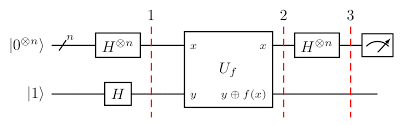
\includegraphics[width=13cm]{images/dj.png}
        \end{center}
        \end{figure}

        \newpage
        
        O algoritmo de Simon consiste em descobrir se uma dada função é 1 para 1 ou 2 para 1 em um cenário que apresenta apenas essas duas possibilidades. Uma função 1 pra 1 significa que um elemento da imagem apresenta apenas um correspondente no domínio enquanto a função 2 pra 1 significa que um elemento da imagem possui dois correspondentes no domínio.
        
        Esse problema foi o primeiro problema quântico em que verificou-se uma solução exponencialmente melhor para um computador quântico em relação ao clássico. A solução quântica é linear enquanto a solução quântica é exponencial.
        
        As principais referências nesse estudo foram o site qiskit.org e o canal do youtube ArturEkert.
    
        O circuito referente a esse algoritmo é:
    
        \begin{figure}[h]
        \begin{center}
        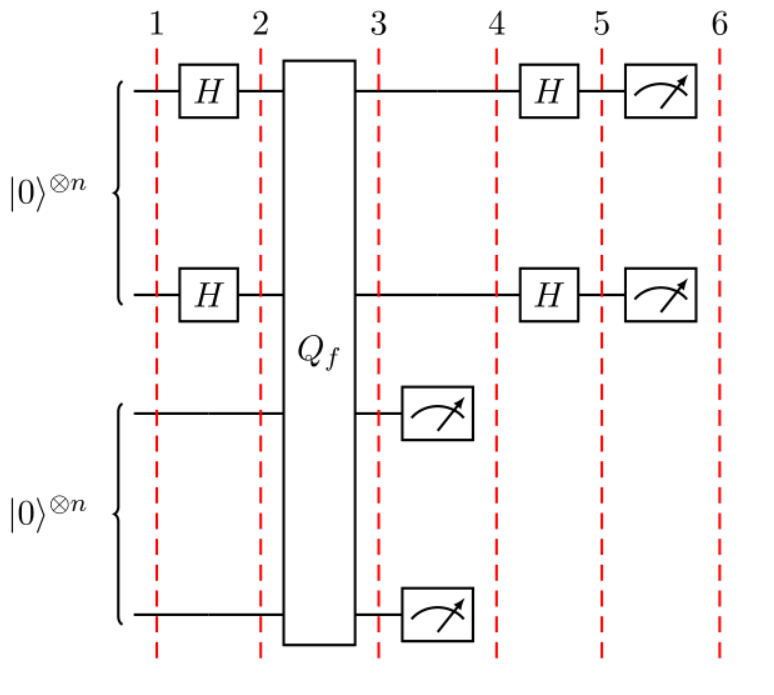
\includegraphics[width=10cm]{images/simons.png}
        \end{center}
        \end{figure}

    \subsection{Comunicação quântica}
        \paragraph{Princípios.}
        Estudei essa parte do tema por meio do artigo ``Quantum internet: A vision for the road ahead-Stephanie Wehner, David Elkouss, Ronald Hanson'' e também pelo material associado à comunicação quântica do XXXVIII Simpósio Brasileiro de Redes de Computadores e Sistemas Distribuídos, produzido pelo professor Antônio Jorge Abelém. 
        
        Primeiramente, a intenção de estudar e tornar realidade uma internet quântica sugere criar novas tecnologias a partir da possibilidade de comunicação quântica entre quaisquer dois pontos do planeta. Nesse ramo, aplicações importantes já foram identificadas, incluindo segurança na comunicação, sincronização do ``clock'', identificação segura de um usuário, economia exponencial em comunicação e também acesso seguro a computadores quânticos remotos na nuvem.

        Dado ambiente de computação quântica, paradigma que apresenta mudanças substanciais em relação ao que foi proposto por Alan Turing, a comunicação quântica aproveita as leis da física quântica para proteger e transmitir informações. Isso pode ser feito a partir da transferência de um estado quântico (emaranhado ou não), da criação de um estado emaranhado ou do uso de um estado emaranhado previamente estabelecido. 

        Nesse contexto, os principais desafios são a dificuldade em criar e manter estados quânticos, a dificuldade em transmitir qubits e a dificuldade em integrar sistemas quânticos com sistemas clássicos.

        \paragraph{Estados de Bell.}
        Antes de abordar outros conteúdos vale ressaltar o que são os estados de Bell. Também conhecidos como pares EPR ou estados maximamente emaranhados, são quatro estados quânticos específicos de dois qubits. Esses estados são nomeados em homenagem a John S. Bell, que os descobriu em 1964. 
        Os estados de Bell são importantes na informação e comunicação quântica porque são maximamente emaranhados, o que significa que seus estados não podem ser descritos independentemente um do outro.Nesses estados, quando um dos qubits emaranhados é medido, o estado do outro qubit é instantaneamente determinado, não importa a distância entre eles. Os estados de Bell têm aplicações na teletransportação quântica, distribuição de chaves quânticas e outros protocolos de comunicação quântica.

        Os quatro estados de Bell são:
        \begin{itemize}
            \item $ \ket{\Phi +} = (\ket{00} + \ket{11}) / \sqrt{2}$
            \item $ \ket{\Phi -} = (\ket{00} - \ket{11}) / \sqrt{2}$
            \item $ \ket{\Psi +} = (\ket{01} + \ket{10}) / \sqrt{2}$
            \item $ \ket{\Psi -} = (\ket{01} - \ket{10}) / \sqrt{2}$
        \end{itemize}
       
        % | Φ + ⟩ = (| 00 ⟩ + | 11 ⟩) / √2
        % | Φ - ⟩ = (| 00 ⟩ - | 11 ⟩) / √2
        % | Ψ + ⟩ = (| 01 ⟩ + | 10 ⟩) / √2
        % | Ψ - ⟩ = (| 01 ⟩ - | 10 ⟩) / √2
            
        \paragraph{Vantagens da comunicação quântica.}
        Por meio da série de vídeos ``Understanding Quantum Information and Computation'' disponibilizadas no canal Qiskit do youtube, além de revisar e entender conceitos introdutórios, pude ver mais profundamente alguns benefícios da comunicação quântica. Primeiramente, estudei o protocolo de teletransporte quântico, método que permite a transferência exata de um estado quântico de um qubit para outro, algo importante já que o estado do qubit não pode ser copiado. Esse protocolo apresenta uma vantagem inicial de que a informação quântica não pode ser verificada no meio de um processo nem copiada, o que é positivo para questões de segurança. Além disso, a propriedade de emaranhamento permite uma comunicação rápida e eficiente, haja vista que tal característica sugere uma correlação que independe da distância entre as duas partículas emaranhadas.

        O vídeo também apresenta o jogo CSHS (Clauser-Horne-Shimony-Holt), que consiste basicamente em dois jogadores, Alice e Bob, que podem se comunicar previamente e após o inicio um árbitro fornece um valor pertencente ao conjunto $\{0,1\}$ aleatoriamente para cada jogador e eles devem devolver para o árbitro um dos dois valores possíveis. Sabendo que os jogadores não podem se comunicar após o início, eles vencem caso o OU exclusivo lógico entre $a$ e $b$ for igual ao E lógico entre $x$ e $y$, sendo $a$ e $b$ as respostas de Alice e Bob e $x$ e $y$ os números enviados pelo árbitro. Perante essas regras, uma comunicação clássica prévia permite que os jogadores ganhem, em média, 75\% das vezes, enquanto utilizando uma estratégia quântica esse índice de vitória sobe para. Tal fato explicita uma vantagem da comunicação quântica a partir da utilização de qubits emaranhados (o que foi feito nesse caso).

        % O circuito referente ao protocolo de teletransporte quântico é:
    
        % \begin{figure}[h]
        % \begin{center}
        % 
\includegraphics[width=10cm]{MAC0215/simons.png}
        % \end{center}
        % \end{figure}
        
        \paragraph{\emph{Entaglement swapping} e \emph{Quantum Key Distribution}.}
        Nesta seção apresentarei dois importantes protocolos que estudei associados à área de comunicação e internet quântica.
        
        \emph{Entaglement swapping} ou troca de emaranhamento é um protocolo de comunicação quântica que permite a criação de entrelaçamento entre duas partes remotas sem nenhuma interação direta. O protocolo requer o uso de dois pares de qubits entrelaçados, referidos como pares de qubits AB e CD, respectivamente.

        O processo de entrelaçamento começa com os dois pares de qubits entrelaçados sendo fisicamente separados e distribuídos para dois locais diferentes, com os qubits A e C enviados para um local e os qubits B e D enviados para outro.
        
        Em seguida, é realizada uma medição nos qubits B e C. Essa medição projeta os dois qubits em um dos quatro possíveis estados de Bell. Dependendo do resultado dessa medição, o entrelaçamento entre os qubits A e D é destruído ou trocado com os qubits B e C.
        
        O \emph{Entaglement swapping} tem implicações significativas para as redes de comunicação quântica, pois permite a criação de entrelaçamento entre partes distantes sem a necessidade de um link de comunicação quântica direta. Isso é especialmente importante para o desenvolvimento de protocolos de comunicação quântica seguros em longas distâncias.

        Segue uma ilustração explicitando como o protocolo funciona:

        \begin{figure}[h]
        \begin{center}
        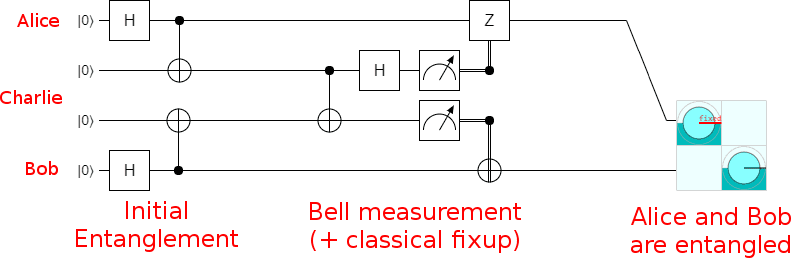
\includegraphics[width=10cm]{images/entanglement-swap.png}
        \end{center}
        \end{figure}

        QKD (\emph{Quantum Key Distribution}) é um protocolo de criptografia quântica que permite a criação de uma chave de criptografia compartilhada entre duas partes que é impossível de ser interceptada por um observador externo. Isso é possível graças aos princípios da mecânica quântica, que permitem a criação de chaves criptográficas que são intrinsecamente seguras.

        O processo de QKD envolve a transmissão de qubits através de um canal quântico, como um cabo de fibra óptica ou um canal de ar, entre duas partes, referidas como Alice e Bob. Esses qubits são usados para gerar uma chave criptográfica compartilhada, que é usada para criptografar e descriptografar mensagens entre as partes.
        
        Durante o processo de QKD, Alice envia uma sequência de qubits para Bob, que mede esses qubits e envia uma resposta a Alice. Essa resposta é usada para corrigir quaisquer erros de transmissão que possam ter ocorrido durante a transmissão dos qubits, permitindo que as partes concordem em uma chave criptográfica compartilhada que é segura contra interceptação.

        Segue uma ilustração explicitando como o protocolo funciona:

        \begin{figure}[h]
        \begin{center}
        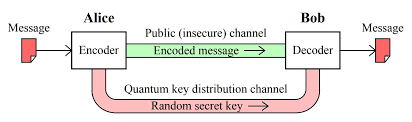
\includegraphics[width=10cm]{images/qkd.png}
        \end{center}
        \end{figure}

        

        \paragraph{Internet quântica.}
        Uma internet quântica consiste em três elementos básicos de hardware quântico. Primeiro precisa-se de uma conexão física que suporte a transmissão de qubits. Em segundo lugar, precisa-se de um meio para conseguir aumentar as distâncias de transmissão. Por fim, necessita-se de processadores quânticos conectados à internet quântica para processar a informação recebida. 
        
        A transmissão de qubits pode ser feita de diferentes maneiras incluindo a fibra óptica, amplamente utilizada em redes de telecomunicações convencionais. No entanto, a fibra óptica convencional não é adequada para a comunicação quântica e, devido a isso, os pesquisadores desenvolveram tipos especializados de fibra óptica, como as fibras de cristal fotônico, projetadas para minimizar a decoerência e suportar a transmissão de qubits. Nesse cenário porém, a taxa de erro na transmissão aumenta quadraticamente com a distância. Outro sistema físico para a transmissão de qubits é a comunicação óptica de espaço livre, que utiliza lasers para enviar informações pelo ar. Essa abordagem tem sido utilizada para estabelecer comunicação entre estações terrestres e satélites em órbita, e tem o potencial de suportar a comunicação quântica por distâncias muito maiores do que a fibra óptica.

        Em ambos os casos, ainda é necessário um meio de ampliar as distâncias entre dois pontos em uma rede de comunicação quântica, o que é feito por repetidores quânticos, que funcionam ampliando e tratando sinais quânticos. Eles são compostos por vários componentes, incluindo processadores de informações. Um dos principais desafios para a construção de repetidores quânticos é a necessidade de preservar as informações quânticas durante a amplificação do sinal. Isso pode ser alcançado usando protocolos de correção de erros quânticos, que visam manter a integridade das informações. No final, a informação é recebida por meio de processadores quânticos que irão tratar a mensagem. 
        
        Um ponto importante a se destacar sugere que, segundo o artigo em questão, uma internet quântica pretende complementar a comunicação clássica e não substituí-la.  

    %\subsubsection{Desafios e perspectivas da área}

    \subsection{Seminários Bern}
        Neste semestre estou participando de um seminário online sediado pela universidade de Bern na Suiça referente ao tema QMN (\emph{quantum mobile networks}). O seminário consiste em apresentações semanais em inglês feitas por alunos da Universidade Federal do Pará, Nanyang Technological University (Singapura),Technical University of Dresden (Alemanha), University of Bern (Suiça), University of Luxembourg (Luxemburgo), University of Massachusetts (Estados Unidos) e University of Reggio Calabria (Itália) sobre os seguintes temas:

        \begin{enumerate}
            \item \emph{Physical Implementations of Quantum Channels in QMNs} 
            \item \emph{Simulation Tools for QMNs}
            \item \emph{Media Access Control in QMNs} 
            \item \emph{Routing in QMNs}
            \item \emph{Performance in QMNs: Capacity, Delay, Buffering} 
            \item \emph{Gossip Protocols in QMNs}
            \item \emph{Age of Information in QMNs}
            \item \emph{Effects of Mobility Patterns on QMN Performance}  
        \end{enumerate}

            
        Os alunos são divididos em grupos de duas a quatro pessoas e cada grupo fica responsável por estudar e fazer uma apresentação sobre um dos temas. Meu grupo, formado por mim e uma aluna da universidade de Bern, ficou com o tema 5. Até o momento os cinco primeiros grupos (o que inclui o meu) se apresentaram.

        % \subsubsection{Physical Implementations of Quantum Channels in QMNs}
        % 

        % \subsubsection{Simulation Tools for QMNs}
        % 

        % \subsubsection{Media Access Control in QMNs }
        % 

        % \subsubsection{Routing in QMNs}
        % 

        % \subsubsection{Performance in QMNs: Capacity, Delay, Buffering}
        % 

    \subsection{Outras atividades realizadas}
        Nesta seção serão descritas outras atividades realizadas durante o período de pesquisa para complementar o estudo.

        Primeiramente, vale ressaltar que os primeiros vídeos da ``qiskit global summer school 2020'' e o site \href{https://qiskit.org}{https://qiskit.org} serviram para revisar e aprofundar os conhecimentos acerca das bases da computação quântica. Por mais que esta não fosse uma referência presente no projeto de pesquisa, devido a qualidade dos vídeos e textos, julgou-se pertinente utilizar este conteúdo. 

        Outro meio que complementou os estudos foram as duas defesas de mestrado de alunos do IME-USP que assiste, ambas sobre computação quântica passando pelos temas mostrados nesse relatório entre outros, como jogos de comunicação. Isso foi realizado de modo a compreender as apresentações dos mestrandos, além de solidificar o conhecimento na área e entender como uma apresentação de mestrado funciona.

        Também assisti 3 apresentações do aluno de mestrado orientado pelo professor Antônio Jorge Abelém (coorientador do projeto). A primeira apresentação foi sobre as bases da computação quântica, a segunda foi uma demonstração de como rodar programas quânticos em computadores quânticos pelo site da IBM e a terceira foi uma introdução à comunicação quântica.
    
        Também, durante o projeto, acompanhei e li algumas notícias que se encaixavam no contexto da pesquisa. Alguns dos temas foram supremacia quântica \footnote{www.nature.com/articles/s41586-019-1666-5}, descobertas na área de comunicação quântica\footnote{beta.nsf.gov/news/tiny-optical-cavities-could-make-quantum-networks-possible}, segurança no contexto quântico\footnote{beta.nsf.gov/news/toward-unhackable-quantum-internet} e prêmios da área. 
        
        % \href{https://www.nature.com/articles/s41586-019-1666-5}{supremacia quântica}, \href{https://beta.nsf.gov/news/tiny-optical-cavities-could-make-quantum-networks-possible}{descobertas na área de comunicação quântica}, \href{https://beta.nsf.gov/news/toward-unhackable-quantum-internet}{segurança no contexto da computação quântica} e \href{https://www.nytimes.com/2022/10/04/science/nobel-prize-physics-winner.html?unlocked_article_code=AAAAAAAAAAAAAAAACEIPuonUktbfqYhlSFUbBybOVtkqqBaLwv7IyrE4w2fkLTqYDC5C3v8UCJPF5EbLY6d5Idsv2jDRDPlwDIgSft0ghOlOIx4qDACyvpqPnJlCLXhv9d3iAG1z0ZmTAfVlqjHnKzjgdLk6zeLk5x7dPmO9D6TYwmRhcFg-2eZtcV-g3HUPxqfXQKUiipQlg6BXVt0tTiwAZSKKo_HqFxx4Xd2GZRne4QAzMPpLDXCRxZXPruJdL3gBTA7OX3h94m0j6NpDONJxPK33LxcoecuWkqwcm8vTEA3ohQWqE9s2-L6Y&smid=nytcore-ios-share&referringSource=articleShare}{prêmios da área}.

    \subsection{Bepe}
    
        Em conjunto com o pedido de renovação associado a este relatório, o bolsista em questão fará a solicitação de um BEPE (bolsa de estágio e pesquisa no exterior), em que o objetivo é aprofundar e direcionar os estudos para a parte de comunicação quântica, mais especificamente, trabalhar com aplicações de \emph{quantum walks} em redes quânticas.

\newpage
    

% \section{Descrição e avaliação do Apoio Institucional recebido no período}
%     O Departamento de Ciência da Computação do IME-USP ofereceu ao aluno todo apoio necessário mesmo mediante a pandemia viral de Covid-19. O aluno contou com uma ótima infraestrutura para realizar seus estudos incluindo serviços de computação e acesso a periódicos. Por fim, os professores do departamento foram sempre muito solícitos em tirar dúvidas e debater tópicos do projeto, em especial os orientadores do mesmo, que 

% \newpage

% \section{Plano de atividades para o próximo período}
%      Nestes seis primeiros meses estudei os princípios da computação quântica, passando pelos principais pilares da área tanto teóricos quanto alguns mais práticos(implementação de programas). Foi iniciado também o estudo na parte de comunicação e internet quântica.

%      Em acordo com o que foi proposto no projeto de pesquisa, o intuito é, com ajuda dos conhecimentos adquiridos até agora, direcionar os próximos trabalhos para a área da comunicação e Internet quântica. O início da pesquisa será baseado nas bases conceituais da área e em seguida tem-se o objetivo de propor uma linha autoral de pesquisa original em Internet Quântica.

%      Na área da comunicação quântica, uma Internet quântica permitirá aplicações que extrapolam o escopo da Internet clássica, principalmente no âmbito da segurança, devido às propriedades da física quântica, que permitem proteger os dados durante a troca de informações e também compartilhar estados quânticos entrelaçados entre duas ou mais partes. No entanto, os sinais quânticos são muito frágeis e não podem ser amplificados ou copiados, pois, para se copiar um qubit, precisaria medi-lo, o que o faria colapsar, inviabilizando o processo desejado. Desafios como este criam uma gama de possibilidades de estudos para resolvê-los e, por conseguinte, ampliam a relevância das pesquisas na área.

%      Dado isso, pretende-se dar continuidade ao cronograma presente no projeto de pesquisa. Os próximos tópicos a serem estudados são inovações recentes na área da comunicação quântica e internet quântica, além de complementar os estudos sobre os princípios da comunicação quântica e continuar alimentando a página do projeto e apresentando seminários. Como mencionado anteriormente, deseja-se nesse período elaborar uma proposta de pesquisa autoral e original sobre o tema protocolos de roteamento para Internet Quântica. 

% \subsection{Cronograma}
% Para exemplificar melhor, segue o cronograma:

% \begin{table}[h]
% \begin{tabular}{|l|l|l|l|l|l|l|}
% \hline
% \begin{tabular}[c]{@{}l@{}}meses\\ ----------\\ tópicos\end{tabular}                                                                              & 7 & 8 & 9 & 10 & 11 & 12 \\ \hline
% Princípios da comunicação quântica                                                                                                                & X &   &   &    &    &    \\ \hline
% Estudos recentes na área da comunicação quântica                                                                                                  & X & X &   &    &    &    \\ \hline
% Internet Quântica                                                                                                                                 &   & X & X & X  & X  & X  \\ \hline
% \begin{tabular}[c]{@{}l@{}}Elaborar uma proposta autoral de pesquisa sobre \\ o tema protocolos de roteamento para Internet Quântica\end{tabular} &   &   &   & X  & X  & X  \\ \hline
% \begin{tabular}[c]{@{}l@{}}Apresentação de seminários para o grupo de \\ pesquisa sobre os assuntos estudados\end{tabular}                        & X & X & X & X  & X  & X  \\ \hline
% Disponibilização do conteúdo estudado no site do projeto                                                                                          & X & X & X & X  & X  & X  \\ \hline
% \end{tabular}
% \end{table}

%  Serão utilizadas as referências que foram descritas no projeto de pesquisa para tais temas. Vale ressaltar que também pretendemos solicitar uma bolsa de estágio de pesquisa no exterior(BEPE) no próximo semestre.
     

\section{Referências Bibliográficas}
    Além de algumas referências citadas durante o relatório em questão o material estudado foi:\\
    
    [Abelem et al. 2020] - Abelém, A. J. G. ; Vardoyan, Gayane ; Towsley, Don . Quantum Internet: The Future of Internetworking. In: Minicursos do XXXVIII Simpósio Brasileiro de Redes de Computadores e Sistemas Distribuídos. 1ed.: SBC, 2020, p. 48-90. doi.org/10.5753/sbc.5033.7.2.\\
    
    [Arute et al. 2019]-Arute, F., Arya, K., Babbush, R. et al. Quantum supremacy using a programmable superconducting processor. Nature 574, 505–510 (2019). doi.org/10.1038/s41586-019-1666-5.\\
    
    [Courtland 2017]-Courtland, R. ‘‘Google aims for quantum computing supremacy; News,’’ IEEE Spectr., vol. 54, no. 6, pp. 9–10, Jun. 2017.\\
    
    [Nielsen 2010] - Nielsen, Michael A., C. I. (2010).Quantum computation and quantum information:  10th Anniversary Edition.  Cambridge University Press, New York, NY,USA.\\
    
    [Portugal et al. 2012] - Uma Introdução à Computação Quântica- Portugal, Renato; Lavor, Carlile Campos; Carvalho, Luiz Mariano; Maculan, Nelson.\\
    
    [Portugal et al. 2019] - Jornada de Atualização em Informática 2019, SBC(Sociedade Brasileira de Computação), capítulo 1, Introdução à Programação de Computadores Quânticos-Renato Portugal, Franklin Marquezino.\\

    [Portugal et al. 2018] - Portugal, R. Quantum Walks, and Search Algorithms. Springer Nature Switzerland AG 2018.\\

    [Wehner et al. 2018] - Wehner, Stephanie, Elkouss, D., and Hanson, R. “Quantum internet: A vision for the road ahead.” Science, 362(1):303, 2018.\\


	\section{Abstract}

    Quantum walks are a powerful algorithmic tool in quantum computing. They have proven to be universal for quantum computing and have provided quantum speed-ups in a myriad of applications. Despite all their generality and properties, quantum walks are simple. In particular, discrete-time coined quantum walks are described by the product of two operators, known as the coin and shift operators, which are sufficient to implement arbitrary quantum algorithms.\\
    This project explores quantum walks in the context of quantum networks. It has been previously demonstrated that quantum walks can be used to control distributed quantum operations in network nodes under the assumption that network nodes have access to ideal quantum gates and memories \cite{controlplane}. This project extends this initial formulation to consider a more physical implementation of the control plane \cite{universalcontrolplane}. For that, we developed simulations of the quantum walk protocol to investigate our implementation approaches.\\


% ---------------------------------------------------------------------------
% \section{Project}
    
%     All the things are in the other overleaf.\\

%     \subsection{Draft}
%     \begin{itemize}
%         \item Quantum gate teleportation (Cnot): \\
    
%         $S_0 = \ket{\psi}\ket{0}\ket{0}\ket{0}\ket{0}\ket{\psi}$\\
        
%         $S_1 = \ket{\psi}\ket{+}\ket{0}\ket{+}\ket{0}\ket{\psi}$\\
        
%         $S_2 = \ket{\psi} \otimes \frac{1}{\sqrt{2}}(\ket{00} + \ket{11})\otimes \frac{1}{\sqrt{2}}(\ket{00} + \ket{11})\otimes \ket{\psi}$\\
        
%         $S_3 = (\alpha\ket{0} + \beta\ket{1}) \otimes \frac{1}{2}(\ket{0000} + \ket{0111} + \ket{1100} + \ket{1011}) \otimes (\gamma\ket{0} + \delta\ket{1})$\\
        
%         $S_3 = \frac{1}{2}(\alpha\ket{0}\ket{0000} + \alpha\ket{0}\ket{0111} + \alpha\ket{0}\ket{1100} + \alpha\ket{0}\ket{1011} + \beta\ket{1}\ket{0000} + \beta\ket{1}\ket{0111} + \beta\ket{1}\ket{1100} + \beta\ket{1}\ket{1011}) \otimes (\gamma\ket{0} + \delta\ket{1})$\\
    
%         $S_3 = \frac{1}{2}(\alpha\ket{0}\ket{0000}\gamma\ket{0} + \alpha\ket{0}\ket{0111}\gamma\ket{0} + \alpha\ket{0}\ket{1100}\gamma\ket{0} + \alpha\ket{0}\ket{1011}\gamma\ket{0} + \beta\ket{1}\ket{0000}\gamma\ket{0} + \beta\ket{1}\ket{0111}\gamma\ket{0} + \beta\ket{1}\ket{1100}\gamma\ket{0} + \beta\ket{1}\ket{1011}\gamma\ket{0} +
%         \alpha\ket{0}\ket{0000}\delta\ket{1} + \alpha\ket{0}\ket{0111}\delta\ket{1} + \alpha\ket{0}\ket{1100}\delta\ket{1} + \alpha\ket{0}\ket{1011}\delta\ket{1} + \beta\ket{1}\ket{0000}\delta\ket{1} + \beta\ket{1}\ket{0111}\delta\ket{1} + \beta\ket{1}\ket{1100}\delta\ket{1} + \beta\ket{1}\ket{1011}\delta\ket{1})$\\
    
%         $S_3 = \frac{1}{2}(\alpha\gamma\ket{000000} + \alpha\gamma\ket{001110} + \alpha\gamma\ket{011000} + \alpha\gamma\ket{010110} + \beta\gamma\ket{100000} + \beta\gamma\ket{101110} + \beta\gamma\ket{111000} + \beta\gamma\ket{110110} +
%         \alpha\delta\ket{000001} + \alpha\delta\ket{001111} + \alpha\delta\ket{011001} + \alpha\delta\ket{010111} + \beta\delta\ket{100001} + \beta\delta\ket{101111} + \beta\delta\ket{111001} + \beta\delta\ket{110111})$\\

%         \item Quantum gate teleportation(swap gate):\\
%         We can do a swap gate using tree cnot gates.
        
%     \end{itemize}

    
%--------------------------------------------------------------------------------------
% \section{Learning}

%     \subsection{Meetings}
%     Clifford operators: In quantum computing and quantum information theory, the Clifford gates are the elements of the Clifford group, a set of mathematical transformations which normalize the n-qubit Pauli group, i.e., map tensor products of Pauli matrices to tensor products of Pauli matrices through conjugation. The notion was introduced by Daniel Gottesman and is named after the mathematician William Kingdon Clifford.[1] Quantum circuits that consist of only Clifford gates can be efficiently simulated with a classical computer due to the Gottesman–Knill theorem. The Clifford group is generated by three gates, Hadamard, phase gate S, and CNOT. (wikipedia) \\
%     Stabilizer states:  they are exactly the states that are reachable from $\ket{0...0}$ using the Clifford gates\\
%     You can perform computation with n instead of $2^n$ complex numbers using pauli strings. A state can be characterized in a unique way with n matrices "M" that $M \ket{\Psi} = \ket{\Psi}$\\
%     For transmission, qubits should be photons\\
%     Google meeting: surface code. Is a technique to do error correction \\
%     Error mitigation has the same objective of quantum error correction but you do not use extra qubits.\\
%     Probabilistic error cancellation. (one possible error mitigation).\\
%     graph states.\\
%     absorption.\\
    
%     \subsection{Interesting}
%     \begin{itemize}
%         \item All quantum operations $E$ on a system of Hilbert space dimension $d$ can be generated by an operator-sum representation containing at most $d^{2}$ elements: $E(p) = \sum\limits_{k=1}^{M}E_k \rho E_k^{\dag}$ , where $1 < M < d^{2}$ . \cite{quantccompquantinfo}

%         \item $tr( A \ket{\psi}\bra{\psi}) = \bra{\psi} A \ket{\psi}$. A is an arbitrary operator.

%         \item You can construct toffoli gates only using cnot gates.
        
%     \end{itemize}


%--------------------------------------------------------------------------------------
\section{The fundamentals of quantum walks, quantum information, and simulation}
    On this section I will present some fundamental concepts that were very important for the research. During the semester at the University of Massachusetts Amherst, I participated in the Quantum Information Systems class as a listener and carrying out all evaluation activities. I will also present a summary of what was taught in each class.\\
    
    \textbf{Important Concepts:}\\
    
    \begin{itemize}
        \item Hilbert space: an inner product space that is complete with respect to the norm defined by the inner product
        
        \item $\bra{\psi}\ket{\phi}$ : inner product.
        
        \item $\ket{\psi}\ket{\phi}$ : tensor product.
        
        \item Normal Operator: An operator A on V is normal if $A^\dag A = A A^\dag$.\cite{portugal}
        
        \item Unitary evolution: An operator $U$ is unitary if $U^\dag U =  UU^\dag = I$ . Unitary operators are normal. They are diagonalizable with respect to an orthonormal basis. Eigenvectors of a unitary operator associated with different eigenvalues are orthogonal. The eigenvalues have unit modulus, that is, they have the form $e^{\imath\alpha}$ , where $\alpha$ is a real number . Unitary operators preserve the inner product, that is, the inner product of $U\ket{v1}$ and $U\ket{v2}$ is equal to the inner product of $\ket{v1}$ and $\ket{v2}$ . The action of a unitary operator on a vector preserves its norm \cite{portugal} . A complex square matrix $U$ is called unitary if the columns of $U$ form an orthonormal set.
        
        \item Hermitian Operator: An operator A on V is Hermitian or self-adjoint if $A^\dag = A$.\cite{portugal}

        \item Positive Operator: A positive operator A is defined to be an operator such that for any vector $\ket{v}$,($\ket{v}$, $A\ket{v}$) is a real, non-negative number. If ($\ket{v}$, $A\ket{v}$) is strictly greater than zero for all $\ket{v} \neq 0$ then we say that A is positive definite. In Exercise 2.24 on this page you will show that any positive operator is automatically Hermitian, and therefore by the spectral decomposition has diagonal representation $\sum_i \lambda_i \ket{i}\bra{i}$, with non-negative eigenvalues $\lambda_i$ . \cite{quantccompquantinfo}
        
        \item Wavefunction: On the quantum computing field, a wavefunction is a function that the x axis corresponds to the basis states and the y axis corresponds to the quantum amplitude of the state.
        
        \item Pure or mixed state:  On a Bloch sphere, pure states are represented by a point on the surface of the sphere, whereas mixed states are represented by an interior point. The completely mixed state of a single qubit is represented by the center of the sphere, by symmetry. The purity of a state can be visualized as the degree in which it is close to the surface of the sphere. In quantum mechanics, the state of a quantum system is represented by a state vector (or ket) $\ket{\Psi}$ . A quantum system with a state vector $\ket{\Psi}$ is called a pure state. However, it is also possible for a system to be in a statistical ensemble of different state vectors: For example, there may be a 50\% probability that the state vector is $\ket{\Psi_{1}}$ and a 50\% chance that the state vector is $\ket{\Psi_{2}}$. This system would be in a mixed state. The density matrix is especially useful for mixed states, because any state, pure or mixed, can be characterized by a single density matrix. 
        
        \item Measurement: Quantum measurements are described by a collection ${M_m}$ of measurement operators. These are operators acting on the state space of the  system being measured. The index m refers to the measurement outcomes that may occur in the experiment. If the state of the quantum system is $\ket{\psi}$ immediately before the measurement then the probability that result m occurs is given by $p(m) = \bra{\psi}M_{m}^{\dag}M_{m}\ket{\psi}$ and the state of the system after the measurement is $\frac{M_{m}\ket{\psi}}{\sqrt{\bra{\psi}M_{m}^{\dag}M_{m}\ket{\psi}}}$ . The measurement operators satisfy the completeness equation, $\sum\limits_{m} M_{m}^{\dag}M_{m} = I$ . The completeness equation expresses the fact that probabilities sum to one: $1 = \sum\limits_{m} p(m) = \sum\limits_{m} \bra{\psi}M_{m}^{\dag}M_{m}\ket{\psi}$ . \cite{quantccompquantinfo}
        
        \item Projective measurement: A projective measurement is described by an observable, $M$ , a Hermitian operator on the state space of the system being observed. The observable has a spectral decomposition, $\sum\limits_m mP_m$ , where Pm is the projector onto the eigenspace of M with eigenvalue m. The possible outcomes of the measurement correspond to the eigenvalues, m, of the observable. Upon measuring the state $\ket{\psi}$, the probability of getting result m is given by $p(m) = \bra{\psi}P_m\ket{\psi}$ .Given that outcome m occurred, the state of the quantum system immediately after the measurement is $\frac{P_m\ket{\psi}}{\sqrt{p(m)}}$. The average value of the observable M is often written $\braket{M} = \bra{\psi}M\ket{\psi}$.\cite{quantccompquantinfo}
        
        \item Orthogonal Projector: An operator P on V is an orthogonal projector if $P^{2} = P\ and\ P^\dag = P$. \cite{portugal}

        \item Fidelity: A second measure of distance between quantum states is the fidelity. The fidelity is not a metric on density operators, but we will see that it does give rise to a useful metric. This  section reviews the definition and basic properties of the fidelity. The fidelity of states $\rho$ and $\sigma$ is defined to be $F(\rho,\sigma) = tr \sqrt{\rho^{\frac{1}{2}} \sigma \rho^{\frac{1}{2}}}$. Fidelity does satisfy many of the same properties as the trace distance. For example, it is invariant under unitary transformations: $F(U\rho U^{\dag}, U\sigma U^{\dag}) = F(\rho,\sigma)$. The fidelity between a pure state $\ket{\psi}$ and an arbitrary state $\rho$ is $\bra{\psi}\rho\ket{\psi}$.\cite{quantccompquantinfo}

        \item Matrix rank: In linear algebra, the rank of a matrix A is the dimension of the vector space generated (or spanned) by its columns. This corresponds to the maximal number of linearly independent columns of A.  %(wikipedia)\\

        \item Quantum circuit depth: The depth of a circuit is a metric that calculates the longest path between the data input and the output. Each gate counts as a unit.  %(medium) \\

        \item With high probability (WHP): In mathematics, an event that occurs with high probability is one whose probability depends on a certain number n and goes to 1 as n goes to infinity. %(wikipedia)\\

        \item Partial trace: It can be calculated as the $\sum_B \bra{\phi_B} \rho_A \otimes \rho_B \ket{\phi_B} = \rho_A \otimes \sum_B \bra{\phi_B} \rho_B \ket{\phi_B}$. In a more clarified way $tr_A(L_{AB}) =\sum_i \langle i|_A L_{AB} |i\rangle_A=\langle0|0\rangle\langle 0|0\rangle (|1\rangle\langle0|)_B+\langle1|0\rangle\langle 1|1\rangle \left(|0\rangle\langle0|\right)_B\\ =(|1\rangle\langle0|)_B$ . 

    \end{itemize}

    \textbf{Quantum walks against Random walks:}\\
    
    When comparing classical random walks with quantum walks the difference appear quickly. The following images make that difference explicit for the one dimensional discrete scenario.

    \begin{figure}[h]
    \centering
    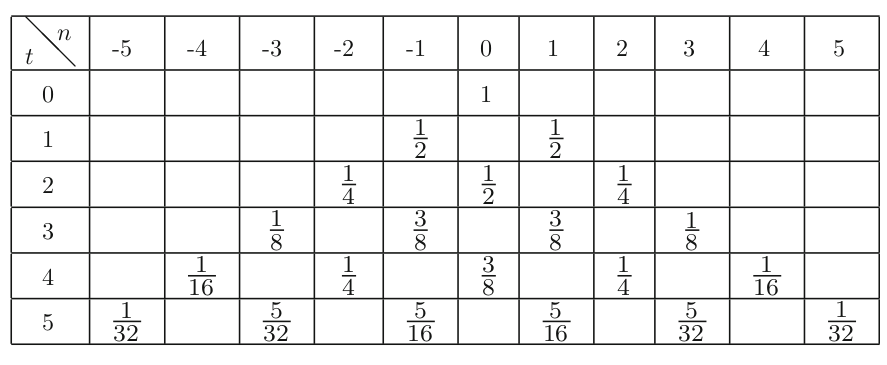
\includegraphics[scale=0.5]{images/rwalks_evolution.png}
    \caption{Random Walk evolution}
    \label{rwe}
    \end{figure}

    \begin{figure}[h]
    \centering
    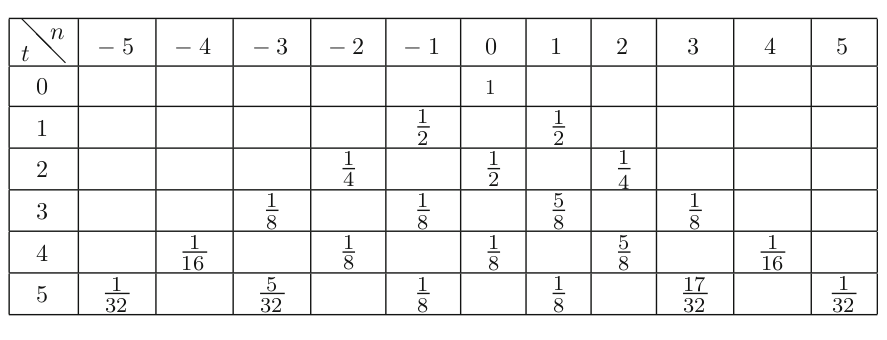
\includegraphics[scale=0.5]{images/qwalks_evolution.png}
    \caption{Quantum Walk evolution}
    \label{qwe}
    \end{figure} 

    \newpage

    If we apply the coin operator followed by the shift operator over and over without intermediary measurements, the quantum correlations between different positions generate constructive or destructive interference, creating a behavior characteristic of quantum walks that is different from the classical behavior.\\

    \textbf{Quantum Information Systems course:}

    \begin{itemize}
    \item {Lecture 1 - Probability and Amplitudes:}\\
    One norm '$|v|_1$' is the sum of the coordinates of the vector. The two norm '$|v|_2$' is the square root of the numbers squares.\\
    Problem: write down the probability matrix of the function f(x) = if (x = 0)  return $1/2 <$ rand()); else return not(x). So the s0 and the matrix are:
    s0 = [0.3 0.7] , matrix p = [0.5 1; 0.5 0].\\
    Stefan made the mirror experience. The expectation did not met so we could not apply classical probability theory for this problem.\\
    $U^{\dag}$ of a unitary operator $U$ is the transpose conjugate of $U$.\\
    You can see the inversibility of matrices as a bijection.\\

    \item {Lecture 2 - Bomb Example:}\\
    Overview to the quantum formalism, that is different from the classical one. It uses complex numbers and the two norm. \\
    The abs(det U) = 1 raises from the fact that two norm is equal to one. Better if you see the definition that the columns of a Unitary form a orthonormal set and then use determinant properties.\\
    Mirror example with a wall compared to the one that does not have one. One path interfere the other, what does not exist in the classical scenario.\\
    Bomb example, when you scan the bomb it explodes (you can interpret this as a barrier that measure only if it is an active bomb). You use those things to, for example, filter some chemical components that are sensitive for the "measure". It is important to say that on those examples the path (top or bottom) is the one qubit state, the fact that is an active or inactive bomb implies only in the measure (it explodes or not).\\

    \item {Lecture 3 - Measurements:}\\
    Measurement of a single qubit in the Z basis, measurement in any basis of "distinct" basis "events", measurement in an arbitrary basis as a Z basis measurement preceeded by a change of basis operation, multi-qubit states and measurement of a single qubit out of a multiqubit state.\\
    Projectors onto a measurement basis state.

    \item {Lecture 4 - Interesting properties:}\\
    Non-commutativity of measurement, global phases do not affect measurement results, distinguishability of states.\\
    Holevo's theorem (1 qubit = 1 bit of accessible information), No Cloning theorem, entanglement, measurement of entangled pairs, quantum information science applications to communication.\\
    Super dense coding is the name used to mention that you can transmit two bits of information using one qubit if you have an entanglement with the other node. There is a theorem  that states that you can not transmit more then two bits of information with only one qubit, even if you have more then one entanglement.\\

    \item {Lecture 5 - Entanglement features:}\\
    On measurements scenario computer scientists use the logical value to describe the measurement and physicists uses the eigenvalues to describe it. \\
    Teleportation protocol. \\
    Introduction to quantum key distribution describing rsa.\\

    \item {Lecture 6 - Quantum key distribution and mixed states:}\\
    Encoding classical information in the x and z basis. \\
    You can detect the eavesdropper.\\
    Ways to distinguish classical mixture of quantum states and pure states.\\
    If you have some mixed state $p_1 \ket{\psi_1} , p_2 \ket{\psi_2}$ the probability of getting the state $\phi$ is: $p_1 |\bra{\phi}\ket{\psi_1}|^{2} + p_2 |\bra{\phi}\ket{\psi_2}|^{2} = p_1\bra{\phi}\ket{\psi_1}\bra{\psi_1}\ket{\phi} + p_2\bra{\phi}\ket{\psi_2}\bra{\psi_2}\ket{\phi} = \bra{\phi}\rho\ket{\phi} = tr(\rho \ket{\phi}\bra{\phi})$ .\\

    \item {Lecture 7 - Homework 1:}\\
    Doubts about homework 1.\\

    \item {Lecture 8 - Partial trace and mixed states:}\\
    Partial trace. It a way to know information about one subsystem knowing that the other subsystem was measured but you do not know the result.\\
    Why the applying the H gate in the perfect mixture result in the same mixed state as you are introducing quantum information in the system.\\
    Every perfect mixture of any orthogonal states are indistinguishable. Meaning that the density matrix will be the same. You can not distinguish a machine that gives you ket plus half of the times and ket minus the other half from a machine that gives you ket 1 half of the times and ket 0 the other half, for example.\\

    \item {Lecture 9 - Quantum algorithms 1:}\\
    We are looking for algorithms that require a polynomial amount of quantum gates.\\
    You can implement all boolean functions with tofolli gates\\
    Types of quantum circuits oracles: (it is easier to do the math if it is a 1:1 mapping, so the circuits are constructed in a way that this occurs. Input and output state are the same length. One way to do that is by making an n + m input and output instead of a n input and a m output) \\
    Deutsch's algorithm: $f(0) = b_0$ and $f(1) = b_1$ and we want $b_0 $xor $b_1$. This is the one bit scenario and for classical we need one query and for quantum we need only one. This can be done using a hadammard gate and a X measurement.\\ 
    Deutsch-Josza's algorithm generalized for an input that is a bit string of length n is very interesting. I saw the reference in Qiskit. \\

    \item {Lecture 10 - Quantum algorithms 2:}\\
    Simon's algorithm: it does not have a clear application but shows quantum advantage. In the classical case you have $O(\sqrt{2^{n}})$ oracle calls trying to find the coliding points(the ones which have the same value of f) and in quantum we have polinomial calls.\\

    \item {Lecture 11 - Non local games:}\\
    P1 P2 and referee game. \\
    Seeing correlations in the bloch sphere in respect of the angles between states. \\
    Correlated and anti correlated. The first means that if one part measure 1 the other part has a higher chance of measuring 1. The second means that if the first part measure 1 the other part has a higher probability of measuring 0.\\    
    Realism: the observation just reveal a information that was already their. Some scientists argue that this is not true because of quantum.\\

    \item {Lecture 12 - Cloning classical information and Simon's algorithm:}\\
    Question 4 of homework 2. The evolution of a Cnot in a quantum and a classical input. \\
    Continues explaining Simon's algorihtm\\

    \item {Lecture 13 - Introduction to Shor's algorithm:}\\
    Rsa encryption to introduce the intuition to learn Shor's algorithm\\
    Multiplicative groups. If you can find the lenght of the group(this is related with p and q if the group is a N group and N = p.q), you can discovered p and q. Shor algorithm does that. \\
    Introduction to the circuit of Shor algorithm\\

    \item {Lecture 14 - Shor's algorithm circuit:}\\
    Quantum fourier transform: $\bra{j} F \ket{i} = \frac{\omega^{i*j}}{\sqrt{2^{n}}}$, where $\omega = e^{\frac{2\pi}{2^{n}}}$ 
    Analysis of which values have a high probability of being measure after applying the quantum fourier transform\\
    When you average in the qft if you do not use full rotation the vlaues sums to a number that is exponentially small compare to the dimension of the fourier transform.\\

    \item {Lecture 15 - Introduction to Grovers algorithm:}\\
    Explanation of some doubts about the midterm exam. \\
    Finish Shors algorithm explaining that with a few queries, with high probability, you will be able to get the period of the function. \\
    Grovers algorithm is based on the negation of the result you want and an averaging function.\\

    \item {Lecture 16 - Finishing Grovers algorithm:}\\
    Intuition using vectors is very nice.\\
    Using a vector that represents $\ket{x^{*}}$, the "number" you want and a vector that is a equally weight sum of all possible states besides $\ket{x^{*}}$.\\
    The algorithm is about reflections in respect to those states (the all possible with the same weight and the all possible besides $\ket{x^{*}}$ with the same weight.)\\
    Getting the unitary operator thinking about the reflection operator is very nice!.\\
    
    \item {Lecture 17 - Physical implementation of quantum hardware:}\\
    Rydberg atom(neural charge atoms); one electron way more excited than the others.\\
    Cavity.\\
    Optical tweezer array.\\
    Trapped Ions.\\
    Chip.\\
    Cooling technologys: 70 kelvin liquid nitrogen cheaper than milk; 4 kelvin liquid helium 100k dollars; 0.015 kelvin liquid helium and isotop cost million dollars.\\
    You can use spin or orbital to be a qubit.\\
    All above works fine at 4 kelvin\\
    Transmons; you have in the middle the actual chip with the low temperature. You need this temperature to make the thermal radiation to not flip the qubit. All the quantum particles are in the small chip in the middles of the "big" device.\\
    Transmons with cavities. Transmons are the operation part and the cavities are storage part.\\
    Nitrogen vacancy center. Generally called as color centers(there are others besides nitrogen). Nice to interact optically and good memory but you can not move the qubits.\\
    Photonics: use to communicate quantum states. Microdisk resonator to trap the light.\\

    \item {Lecture 18 - Noisy channels:}\\
    CPTP - complete positive trace preserving map\\
    The trace out after an environment interaction is a CPTP map.\\
    $\rho ' = tr_{env}(U(\rho \otimes \rho_{env}) U^{\dag}) = \sum_i E_i \rho E_i^{\dag}$ , where $E_i = \bra{e_i} U \ket{e_0}$\\
    The above expression considered the environment as a pure state $\ket{e_0}\bra{e_0}$.\\
    Pauli channel.\\
    Classical linear binary code.\\  

    \item {Lecture 19 - Numerical examples of CEC and QEC:}\\
    When you are looking for a family of codes the graph of logical error against physical error becomes a non continuous graph where the logical error is zero before a threshold and one after this value.\\
    One constrain in qec is that you can not destroy superposition while doing the error correction.\\
    Steane's 7 qubit code\\
    Shors's 9 qubit code\\

    \item {Lecture 20 - Stabilizer States:}\\
    You can keep track of the set of observables that corresponds uniquely to one state.\\
    You can associate this with the parity check matrix.\\
    Multiple qubits measurements.\\

    \item {Lecture 21 - More on Stabilizer States:}\\
    More of observables.\\
    You can have n observables constrains to represent a n qubit state.\\
    The thing is that you can not do that for all the states(clifford operations).\\
    You can think that the observables are dividing the space and then you have a set of n observables that divides the initial space till you have only one state.\\
    The observables HAVE to comute, because this is the quantum constrain of one observables to not delete the information provided by the previous observable.\\
    Some network protocols, teleportation, superdense coding, can be simulated efficiently in a classical computer using the stabilizer formalism.\\

    \item {Lecture 22 - Stabilizer Formalism Evolution:}\\
    The set $\{ Z\mathds{1}\mathds{1}, ZZ\mathds{1}, ZZZ\} $ represents the state $\ket{000}$.\\
    To know that you think about the space that each of those three observables are spanning. For each observable you need to think of the hole multi qubit system. For example, the observable $ZZ\mathds{1}$ does NOT span $\{\ket{0}\} \otimes \{\ket{0}\} \otimes \mathds{C}^{2}$, it span $\{\ket{00}, \ket{11}\} \otimes \mathds{C}^{2} $ \\
    The evolution of the set of pauli strings can be done simply by doing $US_iU^{\dag}$, where $S_i$ is one of the pauli strings(you that for every peuli strings).\\

    \item {Lecture 23 - More on Stabilizer Formalism Evolution:}\\
    With particular unitary operations you can do the evolution efficiently. \\
    You keep track of a binary string.\\
    You have an X and a Z part of this binary string. $I = (0,0), X = (1,0), Z = (0,1) and Y = (1,1)$, where the first part is the X part and the second is the Z.\\

    \item {Lecture 24 - Finish Stabilizer States and Introduce Useful Error Correcting Codes:}\\
    The unitary used to evolve a stabilizer state to another stabilizer state need to be clifford, meaning that $U$ maps a pauli operator to a pauli string. That is a big constraint because it is not every unitary that satisfies this.\\    
    Examples of stabilizer mapping (convert the exponentially big unitary to the polinomial transformation on the bitstring space).\\
    On real hardware so far you can only make operations between near neighbors qubits.\\
    Introduction to surface codes. They use the information on given on the line above.\\

    \item {Lecture 25 - Useful error correcting codes:}\\
    Torus code with x and z multiple qubits measurements (I think it is surface code).\\
    The center z measurement it is redundant so if you count it gone leave with to degrees of freedom. (k = 2, two logical qubits encoded).\\
    You can turn the torus into a surface (the algebra gets a little bit more complicated).\\
    This type of code is good for the hardware that we have now (with lattices).\\
    Ldpc codes have a lower overhead but there is no hardware now that can implement it because we do not have long range connectivity between qubits now.\\
    You perform the z correction and the x correction separately.\\
    Use minimal weight perfect matching to correct the syndrome errors.\\

    \item {Lecture 26 - Correlation:}\\
    Chsh game.\\
    Quantum do better than classical (85 \% against 75\%.\\
    You can have $100\%$ if you have a correlation stronger than quantum, but they are not physically feasible.\\
    If quantum correlation were stronger that they actually are we would have a huge gain in cryptography.\\
    Non-signaling theory.\\
    We have local correlations (classical), quantum correlation and Non-signalling correlations (mathematical approach having only the non instantaneous communication constrain).\\

    \item My grades on the course: \\
    HW1: 37/37\\
    HW2: 43/43\\
    MIDTERM EXAM: 26/27\\
    HW3: 29/30\\
    HW4: 13/13\\
    HW5: 37/38\\
    FINAL EXAM: 44/44\\
    HW stands for homework.\\
    
    \end{itemize}

    \textbf{Examples of quantum noise, a very important subject for the hole field:}\\
    
    \begin{itemize}
        \item Bit flip: The bit flip channel flips the state of a qubit from $\ket{0}$ to $\ket{1}$ (and vice versa) with probability $1 - p$. On the Bloch sphere representation you can see that the states on the $\hat{x}$ axis are left alone, while the $\hat{y}-\hat{z}$ plane is uniformly contracted by a factor of $1 - 2p$. 
        
        \item Phase flip: The phase flip channel has operation elements $E_0 = \sqrt{p}\ I , E_0 = \sqrt{1 - p}\ Z $. On the Bloch sphere, the states on the $\hat{z}$ axis  are left alone, while the  $\hat{x}-\hat{y}$ plane is uniformly contracted by a factor of $1 - 2p$.

        \item Bit-phase flip: The bit-phase flip channel has operation elements $E_0 = \sqrt{p}\ I , E_0 = \sqrt{1 - p}\ Y$, where $\ Y = \imath X Z $. On the Bloch sphere, the states on the $\hat{y}$  axis are left alone, while the $\hat{x}-\hat{z}$ plane is uniformly contracted by a factor of $1 - 2p$.

        \item Depolarizing channel: The depolarizing channel is an important type of quantum noise. Imagine we take a single qubit, and with probability p that qubit is depolarized. That is, it is replaced by the completely mixed state, $I/2$. With probability $1 - p$ the qubit is left untouched. The state of the quantum system after this noise is  $\varepsilon (p) = \frac{pI}{2} + (1- p)\rho$. On the Bloch sphere, the entire sphere contracts uniformly as a function of p. \cite{quantccompquantinfo}
        
        \item Amplitude damping: In this case, the $E_1$ operation changes a $\ket{1}$ state into a $\ket{0}$ state, corresponding to the physical process of losing a quantum of energy to the environment. $E_0$ leaves $\ket{0}$ unchanged, but reduces the amplitude of a $\ket{1}$ state; physically, this happens because a quantum of energy was not lost to the environment, and thus the environment now perceives it to be more likely that the system is in the $\ket{0}$ state, rather than the $\ket{1}$ state. On the Bloch sphere, the entire sphere shrinks towards the north pole, the $\ket{0}$ state. \cite{quantccompquantinfo}
        
        \item Phase damping: A noise process that is uniquely quantum mechanical, which describes the loss of quantum information without loss of energy, is phase damping. A very simple model for this kind of quantum noise is the following. Suppose that we have a qubit $\ket{\psi} = a \ket{0} + b \ket{1}$ upon which the rotation operation $Rz (\theta)$ is applied, where the angle of rotation $\theta$ is random. The random phase kicking causes the expected value of the off-diagonal elements of the density matrix to decay exponentially to zero with time. That is a characteristic result of phase damping. \cite{quantccompquantinfo}
        
    \end{itemize}

 
%--------------------------------------------------------------------------------------
\section{Quantum walk algorithms and their implementations}
    
    In this section, is presented the two mainly important quantum algorithms for our research.\\
    
    \textbf{Quantum Walk Control Plane \cite{universalcontrolplane}:}\\
    
    Quantum Walks Utility in this scenario:\\
    
    The protocol employs a quantum walk as a quantum control signal to execute distributed quantum operations. We generalize the discrete-time coined quantum walk model, which incorporates the interaction between a quantum walker system in the network graph with quantum registers inside the network nodes. The protocol abstracts hardware implementation and the transmission of quantum information through channels. The propagation of the walker system across the network represents the transmission of the control signal, while the application of coin operators integrates interactions between the control layer and the quantum registers. \cite{controlplane}\\
    
    
    Mathematical Background:\\
    
    Consider a directed graph  $G = (V,E)$ obtained from a non-directed graph by introducing two directed edges for each initial one. The sets $N^{+}(v) \subseteq V and N^{-}(v) \subseteq V$ denote the sets of outward and inward neighbors of $v$, respectively.\\
    A complex vector in a Hilbert space $Hw \subseteq Hv \otimes Hc$  evolves through a discrete-time coined quantum walk on graph $G$, defined by the graph structure. The vertex space $Hv$ it is used to codify the vertices of the graph by assigning to each vertex a basis vector of $Hv$, which has dimension $|V|$. The coin space $Hc$ denotes the degrees of freedom of the walker(possible movements for the walker) and has a dimension given by the maximum degree of the graph $D = max{d(v): v \in V}$. The basis for $Hw$ is ${\ket{v,c} : v \in V, c \in Cv}$ , where $Cv = {0, ... , d(v) -1}$ is the integer set for the number of outward edges of a node v. \\
    The basis for the spaces $Hc$ and $Hv$ are denoted as ${\ket{c}}$ and ${\ket{v}}$, respectively. Assuming $\ket{\Psi(t)}$ is the walker wavefunction at discrete time instant $t$, the evolution of the quantum walk is given by the action of two unitary operators $S: Hw \to Hw$ and $W: Hw \to Hw$ on the system state vector $$\ket{\Psi(t+1)}= SW\ket{\Psi(t)}$$\cite{relationship}
    
    Coin operator:\\
    The walker's degrees of freedom are affected by the coin operator $(W)$. The general form of the coin operator is represented by:\\
    $$W = \sum_{v \in V} \ket{v} \bra{v} \otimes Wv$$ where $Wv$ is a unitary operator. The coin operator mixes the amplitude of a particular state $\ket{v,c}$ with states $\ket{v,c'}$ such that $c, c' \in Cv$, which are the degrees of freedom of the same vertex. \cite{equivalence}\\
    
    Shift operator:\\
    The shift operator, also known as the swap operator $(S)$, is responsible for moving the mixed amplitudes generated by the coin operator $W$ to outward edges. To define the operator, we introduce the function$ \eta: V \times C \to V$, which maps outward edges to outward neighbors of each vertex. Thus, for a vertex v and an index $c, \eta(v, c)$ denotes the c-th outward neighbor of $v$, which we denote by $u$. Additionally, we introduce $\sigma: V \times V \to C$, which maps an inward edge of a vertex to one of its outward edges.\\
    The action of the shift operator is then formally defined as follows: for a state vector $\ket{u,c}$, the shift operator transforms it into $\ket{\eta(u,c), \sigma(u,\eta(u,c))}$. Note that $\eta$ and $\sigma$ can be defined arbitrarily as long as the operator remains unitary and respects the graph edges. In fact, different choices of $\eta$ and $\sigma$ can lead to different dynamics of state amplitudes. \cite{equivalence}\\

    \textbf{Grover's graph search:}\\

        Getting the idea of amplitude amplification provided by Grover's algorithm, they build a Grover's search on a graph. This algorithm aims to find a node on a graph starting at a random position. It is important to mention that it is better than any classical approach. After studying it on \cite{portugal}, it brought us the idea of using this in our research by using it on a network search. We did not have time to explore this, but it could be a future work.\\
    

%--------------------------------------------------------------------------------------
\section{Simulation development and experiments}

    My first experiment was to develop a 1-dimensional quantum walk simulation in the Julia programming language. It uses the Hadammard gate as a coin. It was based on the recursion equations for one dimension discrete coined quantum walk in \cite{portugal}. It was good to get familiar with the programming language because the quantum network simulator we used later (QuantumSavory) was written in Julia.\\

    We also wrote a program in Python to try to find the remote gate circuit with the following logic:
        
    We need a unitary $U$ such $U: input \to output$. \\
    $input = \ket{\psi} \otimes (\frac{1}{\sqrt{2}}(\ket{00} + \ket{11}))^{\otimes n}$\\
    $output = \sum_{k} \sqrt{\alpha_{k}} U_{k} \ket{\psi}\ket{k} $, where $U_{k}$ is the error associated with the output $\ket{k}$. \\
    
    Because of the non locality constrain $U$ must be decompose as $U_a \otimes U_b$, meaning that $U_a$ acts only on the qubits in one node and $U_b$ acts only on the qubits on the other node.\\

    Finally, to compare the two approaches to the problem explained in the next section, we start programming a simpler Python simulation using fixed probabilities for the events. We are also working on a network simulation using the QuantumSavory simulator. It is essential to mention that we have yet to get conclusions on those two simulations because we are still working on them.
    
    
%--------------------------------------------------------------------------------------
\section{Refinements to the quantum walk protocol}

    The research goal was defined as implementing the quantum walk protocol described on \cite{controlplane}. By implementation, we mean a go from the logical approach to a more physical approach, including encoding considering the actual physical qubits and showing how we would perform the operations considering the non-locality. More explanations and details about the model are on \href{https://interscity.org/quantum-internet/}{https://interscity.org/quantum-internet/}, where it is a presentation about the quantum walk control plane implementation.\\

    \textbf{Linear Approach}
    \begin{itemize}
        \item The linear approach means that we can use $O(|V|.d_{max})$ qubits,  where $d_{max}$ is the maximum degree of freedom of a node.
        \item Use one qubit to encode each edge.
        \item We used one hot encoding to encode the logical qubits on the physical qubits.
        \item A controlled operation between two nodes needs a number of qubits proportional to the number of vertex in this approach.
        \item The shift operation (swap teleportation gate in this case) can not be done with less then two EPR pairs.
        \item The circuit used to do the shift operation is on \hyperlink{https://algassert.com/post/1717}{https://algassert.com/post/1717}. We programmed and tested this circuit using qiskit.

        % \item What we think is good to find a 1 EPR pair circuit for swap teleportation:\\
        
        % We need a unitary $U$ such $U: input \to output$. \\
        % $input = \ket{\psi_1}\ket{\psi_2} \otimes \frac{1}{\sqrt{2}}(\ket{00} + \ket{11}) $\\
        % $output = \sum_{ij} \sqrt{\alpha_{ij}} U_{ij} \ket{\psi_2}\ket{\psi_1}\ket{ij} $, where $U_{ij}$ is the error associated with the output $\ket{ij}$ \\
        % Because of the non locality constrain $U$ must be on the form $U = U_{1x3} \otimes U_{2x4} $.\\   
        
    \end{itemize}

    \textbf{Logarithmic Approach:}\\
    \begin{itemize}
        \item The logarithmic approach means that we can use $O(|V|.lg(d_{max}))$.
        \item Use the $lg(d(v)+1)$ qubits in each node, where $d(v)$ is the degree of freedom of $v$. 
        \item Same encoding for edges $(u,v)$ and $(v,u)$.
        \item Edges $(u,v)$ and $(v,u)$ are in different nodes.
        \item State $\ket{0...0}$ in a node means that the walker is not on this node. State $\ket{1..1}$ is associated with the self-loop.
            
    \end{itemize} 

    \textbf{Tradeoff between qubits, time and circuits:}\\ 

        Given that the time to execute a shift is negligible if we have an epr pair, both approaches can be done with parallel shifts. The difference is that for the logarithmic approach we need more epr pairs to perform each shift, probably a number associated with the number of qubits used in the encoding. \\

        To do the shift you need the number of epr pairs to do one shift times the number of edges. On the linear approach we need two epr pairs per shift and on the logarithmic approach we do not know yet.\\

        To perform parallel shifts we need more qubits to have more epr pairs at the same time and to perform sequential shifts we have a time delay because we have to wait one operation to start attempting to establish the others epr pairs.\\

    \textbf{Shift Operation}:\\

        To perform the Shift operation we need to do one shift for each edge. That introduces a tradeoff between number of bell pairs and time.\\

        If we do all the shifts at the same time we will need $O(E.b(e))$ epr pairs, where $b(e)$ is the number of bell pairs needed to do a shift considering the current encoding. If we do less qubits we will spend more time to perform the operation since we gonna use the same qubits to make different epr pairs (add the time of stablishing a bell pair between two nodes).\\

        In a two dimensional lattice, the minimum number of shift qubits in each node is $b(e)$, and using that, it seems that you need $O(n)$ rounds of shifts on a $n_xn$ lattice.\\

    \textbf{Branches:}\\

        What we called uncoupled system is the entire qubit system into two groups: encoding qubits and the operation qubits(epr pairs). Given that, we can work with three branches since we can use less epr pairs if we perform sequential shifts. 3 because it does not make sense to analyse the linear encoding with sequential shifts because the parallel version is also asymptotic linear.
    
    \begin{enumerate}
        \item Linear encoding with parallel shift
        \item Logarithmic encoding with sequential shift
        \item Logarithmic encoding with parallel shift
    \end{enumerate}

    \textbf{Comparison between the two approaches:}\\
    
    \begin{tabular}{|c | c | c|} 
     \hline
     \textbf{Modeling details} & \textbf{Linear} & \textbf{Logarithmic} \\
     \hline
     required encoding qubits & $O(|V|d_{max})$ & $O(|V|lg(d_{max}))$ \\ 
     \hline
     coin operation & trivial & trivial\\ 
     \hline
     shift operation & remote swap & selected swap/non trivial\\
     \hline
     encoding qubits per shift & one & $lg(d_{max})$ \\
     \hline
     operation qubits per shift & two & $O(lg(d_{max}))^{*}$\\
     \hline
     one node shift & parallel & sequential or parallel(time is negligible) \\  
     \hline
    \end{tabular}\\ \\

        
    \textbf{Notes about the project:}\\
    \begin{itemize}
    
        \item We can not do the swap teleportation gate using less than 2 epr pairs.The proof relies on the fact that with a remote swap we can create two remote epr pairs, so it must need two epr pairs to do that (\hyperlink{https://journals.aps.org/pra/pdf/10.1103/PhysRevA.64.032302}{link to the paper}).\\

        \item Quantum Error Correction (QEC) should not do better in the qw control plane. We do not know if quantum error correction is better for the quantum walk protocol then for the protocol that just teleport the gate to the end node. But, as we have the overhead on the resources it should be worse.\\
        
        \item Simulation aspects:
        \begin{itemize}
            \item Qubits being used.
            \item Sequential shift or parallel.
            \item Consider time decoherence.
            \item Consider fidelity.
        \end{itemize}

    \end{itemize}

    Clearly we went through some papers during the research. Here I will mention some of them that we analyze: Routing entanglement in the quantum internet \cite{routing_entanglement}, Experimental Implementation of Quantum Walks on IBM Quantum Computers \cite{experimental}, \href{https://quantumai.google/cirq/experiments/quantum_walks}{Google quantum AI about quantum walks} and Implementation of quantum random walk on a real quantum computer \cite{implementation}.

%--------------------------------------------------------------------------------------
\section{Design the outline of a scientific paper}

    After the time at the University of  Massachusetts Amherst, we gonna write and publish a paper with the following topics:

    \begin{itemize}
        \item Introduction considering \cite{universalcontrolplane}.
        \item Linear approach.
        \item Logarithmic approach.
        \item Comparison between the two approaches.
        \item Conclusion considering future improvements on what was done.
    \end{itemize}

    It is important to remember that in this process, we use simulations and coding that we will show and explain in the paper. Also, we may include quantum error correction or other topics in the paper.\\

%-----------------------------------------------------------------------
% \section{Papers}
%     Here are some papers we went through that may have yet to appear. For each one of those, we mention important aspects of the paper. 
    
%     \begin{enumerate}
    
%         \item \textbf{Universal Quantum Walk Control Plane for Quantum Networks \cite{universalcontrolplane}:}\\
%         If the walker is in a state that represents a certain edge actually the walker is in the node that the edge is going out. \\
%         To represent a basis vector (an edge) you only need qubits on the nodes that this edge "touch".\\
%         The number of qubits that the coin space need is log of the degree of freedom of the node that have the max degree of freedom among all nodes.\\
%         The coin operator depends on the minimum path p chosen.\\
%         The shift operator as it is described can be modeled to any other shift operator by just doing another coin operation.\\
    
%         \item \textbf{Routing entanglement in the quantum internet \cite{routing_entanglement}:} \\
%         It is common that all the nodes know the topology.\\
%         Ultimately one would like to develop explicit and efficient practical quantum routing protocols that employ quantum operations implemented via lossy and noisy devices, while only requiring local link-state knowledge and limited knowledge of the global network topology.\\
%         Entanglement rate. What is ebits? The rate is associated with the amount of entanglement you can create per time. The word per mode in this context is associated with the frequency of the transmission (you can transmit in different modes in parallel). An ebit is an entanglement bit. \\
%         The number of memories in each node is equal the summation over all neighbors of vertex v of how many parallel channels you have with each node.\\
%         Each time slot you try every external connection at the same time\\
%         The goal is to find the optimal strategy for each repeater node in order to decide which locally held qubits to attempt BSM(s) on during the internal phase of a time slot, based ideally only on knowledge of the outcomes (success or failure) of the nearest neighbor links, i.e., local link-state knowledge, during the respective preceding external phases. We will assume that each repeater node is aware of the overall network topology, as well as the locations of the K Alice-Bob pairs. The goal of the optimal repeater strategy wil  l be to attain the maximum entanglement-generation rate or the maximum rate-region for multiple flows. \\
%         Manhattan distance is a metric in which the distance between two points is the sum of the absolute differences of their Cartesian coordinates. In a simple way of saying it is the total sum of the difference between the x-coordinates and y-coordinates. (medium.com) \\
%         Recall that the rate along a length k path is $p^{k}q^{k-1}$, where p is proportional $\eta$ is the transmissivity of each link. In the network case, when p $>$ pc and $q = 1$, we find that the pk portion of the rate expression becomes immaterial for scaling with Alice-Bob distance. This behavior can be explained by percolation theory: in a large lattice in this regime, the probability of a connected path between Alice and Bob along successful external links in each time-slot approaches a non-zero constant as the Alice-Bob separation is increased.\\
%         The alfa in the real probability of getting a external link is close to 0.3 and the distance is in km\\
        
%         \item \textbf{Experimental Implementation of Quantum Walks on IBM Quantum Computers:}\\
%         It is about a coinless implementation of a quantum walk (staggered quantum walk model)\\
    
%         \item \textbf{\href{https://quantumai.google/cirq/experiments/quantum_walks}{Google quantum AI about quantum walks:}}\\
%         The process of the quantum walk isn't that much different from its classical counterpart, although the observed results of the two processes have many differences. First, let us motivate the creation of a QW. The idea is that when one performs analysis on a classical random walk, you can find that $\sigma^{2} \sim T$ , where is the standard deviation of the random walk's probability distribution, and is the number of time-steps of the random walk. For the quantum walk, we can see that $\sigma^{2} \sim T^{2}$. In other words, the standard deviation grows at a quadratically faster rate. At a high level, this signifies that the quantum walker "spreads out" quadratically faster than the classical one, showing that the process of a QW is quadratically faster than its classical counterpart. \\
%         This paper explain how to implement the coin and shift operators using cnots. \\
    
%         \item \textbf{Implementation of quantum random walk on a real quantum computer:}\\
%         Citation: Warat Puengtambol et al 2021 J. Phys.: Conf. Ser. 1719 012103\\
%         They used a way of constructing multi controlled qubit toffoli gates using ancillas between every controled qubit


%     \end{enumerate}

%------------------------------------------------------
\section{Future work}

    To disseminate and transfer the knowledge acquired during the BEPE fellowship after returning to the country, I will work on the mentioned paper, written collaboratively with Professor Don Towsley's group at UMass and the Brazilian advisors. I will also participate in meetings of the IME-USP Software Systems group meetings, giving seminars to disseminate the knowledge acquired and sharing his project experiences in collaboration with experienced foreign researchers. It is worth mentioning that during the period in Massachusetts and right after coming back to Brazil, I gave presentations about quantum information and my research to my supervisor, my cosupervisor, and his students from the Federal University of Pará (they are together on the project \href{https://bv.fapesp.br/pt/auxilios/109781/protocolos-de-roteamento-para-internet-quantica/}{https://bv.fapesp.br/pt/auxilios/109781/protocolos-de-roteamento-para-internet-quantica/}).


	\section{Resumo do projeto proposto}
    A computação quântica nasceu a partir da ideia de criar uma máquina capaz de simular sistemas quânticos mais complexos, proposta pelo físico Richard Feynman e pelo matemático Yuri Manin. O esforço para tais simulações em computadores clássicos cresce exponencialmente em função do tamanho do sistema, o que as inviabiliza para qualquer problema de tamanho interessante. Além desse foco, estudos na área de algoritmos também obtiveram sucesso com a computação quântica, em que algoritmos consideravelmente mais rápidos do que os clássicos já foram propostos, como o algoritmo de Shor para a fatoração de números.
    
	Destaca-se também, o fato de que a computação quântica é um objeto de estudo com uma gama de novas possibilidades a serem exploradas, o que a torna mais instigante e promissora. No cenário atual, empresas como a Google e a IBM, destaques nesse ramo, possuem máquinas quânticas funcionais, que demonstram a grande relevância desse estudo. Alguns dos desafios encontrados no trabalho de aprimorar tais computadores são aumentar o número de qubits (unidade básica de memória de um computador quântico), diminuir ruídos e aumentar o tempo de coesão (tempo de duração dos fenômenos quânticos para executar um algoritmo).
 
	Nesta iniciação científica, motivado pelo que foi apresentado, o bolsista, durante o primeiro ano, estudou de forma sistemática os principais conceitos da Computação Quântica e da Comunicação Quântica. Após adquirir a base do conhecimento na área, o bolsista realizou um BEPE (Bolsa de Estágio e Pesquisa no Exterior) na Universidade de Massachusetts em Amherst, onde avançou significativamente com a pesquisa ao estudar mais profundamente o assunto e propor a implementação de um plano de controle distribuído para redes quânticas utilizando passeios quânticos. A contribuição final do projeto foi um artigo que descreve duas codificações propostas para o plano de controle em questão, além de conter uma análise do problema e uma comparação dentro do que foi proposto. 
 
    Em acordo com o que é demandado pela FAPESP, parte dos trabalhos realizados estão disponibilizados publicamente no website do projeto (\href{https://interscity.org/quantum-internet/}{https://interscity.org/quantum-internet}).



\section{Realizações do período}
    No período referente a este relatório final do projeto de título "Computação e Internet Quântica", os trabalhos se relacionaram com a produção de um artigo e a disseminação de conhecimento associado a Computação Quântica e a Redes Quânticas.

    O andamento do projeto ocorreu em acordo com o que foi proposto no cronograma descrito no projeto de pesquisa apresentado para a FAPESP sem atrasos. Nenhum assunto foi negligenciado e em acordo com isto, os tópicos de trabalho durante o período em questão foram:
    \begin{enumerate}
        
        \item Refinamento do trabalho realizado no BEPE
        \item Elaboração do artigo
        \item Submissão e apresentação do artigo
        \item Disseminação do Conhecimento por Meio de Palestras
    \end{enumerate}
    
    Apresentarei a seguir o que foi trabalhado em cada tópico.
    
    Primeiramente, o trabalho desenvolvido em Massachusetts, onde foram propostas duas codificações para o plano de controle presente no artigo \cite{universalcontrolplane}, foi submetido a um processo meticuloso de refinamento e revisão. Adicionalmente, foram incorporadas discussões importantes que aprofundaram a análise dos tradeoffs envolvidos. Nessa parte, aprofundamos a discussão de fatores como a divisão dos qubits utilizados na implementação do protocolo em dois grupos, o conceito de rounds associado a execução da operação de shift no protocolo e a possibilidade de paralelização de operações em duas partes do protocolo. Esses refinamentos foram essenciais para a elaboração do artigo científico, permitindo uma compreensão mais detalhada dos compromissos entre desempenho e complexidade de operações no protocolo. As discussões adicionadas proporcionaram uma base sólida para a interpretação dos resultados e a exploração de novos caminhos de pesquisa.
    
    Após o refinamento apresentado acima, o tempo de trabalho foi dedicado para a elaboração do artigo científico de título ``Distributed Quantum Walk Control Plane Implementation'', a principal colaboração científica do projeto. O artigo foi revisado e melhorado diversas vezes de modo a apresentar uma estrutura concisa e coerente matematicamente. Após sua confecção, o artigo foi submetido e aprovado para apresentação no I Workshop de Redes Quânticas presente no XLII Simpósio Brasileiro de Redes de Computadores e Sistemas Distribuídos (SBRC 2024), que ocorreu no dia 20/05/2024 na Universidade Federal Fluminense.
    
    No artigo, abordamos o problema da implementação do plano de controle em processadores quânticos. Apresentamos duas maneiras de mapear a descrição lógica do protocolo \cite{universalcontrolplane} para qubits nos nós da rede: a codificação linear e a codificação logarítmica. Descrevemos o número de qubits necessários em cada nó, juntamente com uma descrição dos operadores para ambos os métodos propostos. Finalmente, apresentamos uma análise teórica inicial sobre o desempenho das implementações propostas, que mostra um trade-off entre os recursos da rede usados para controle e o tempo necessário para concluir as operações. Além disso, vale ressaltar que o artigo permite diversas possibilidades de continuidade da pesquisa. Entre essas possibilidades, destacam-se o aprofundamento das simulações para comparar as codificações propostas e o estudo das possíveis aplicações práticas para o protocolo desenvolvido. 
    
    O artigo foi apresentado no Rio de Janeiro, durante o I Workshop de Redes Quânticas presente no SBRC 2024. A apresentação foi bem recebida pela comunidade científica, e o artigo foi agraciado com uma menção honrosa, equivalente ao segundo melhor artigo do workshop. Este reconhecimento ressalta a relevância e a qualidade do trabalho desenvolvido, dando crédito para a contribuição feita por este projeto.
    
    Também em acordo com o que foi proposto pelo cronograma, visando disseminar o conhecimento adquirido e promover o debate acadêmico, foram realizadas palestras direcionadas ao orientador, coorientador e alunos. Além disso, foram feitas apresentações para o grupo de sistemas do Instituto de Matemática e Estatística da Universidade de São Paulo (IME-USP).
    
    Estas palestras abordaram tópicos relacionados à informação quântica, com destaque para os conteúdos desenvolvidos no artigo científico. Os principais tópicos foram: introdução a passeios aleatórios, introdução a passeios aleatórios quânticos, explicação da modelagem presente em \cite{universalcontrolplane} e a apresentação detalhada do trabalho desenvolvido em Massachusetts. Essas atividades de disseminação foram fundamentais para promover o entendimento de conceitos de redes quânticas na comunidade acadêmica, incentivando o desenvolvimento de novas pesquisas e colaborações na área. É importante mencionar que as apresentações foram disponibilizadas no site do projeto.
    
    Desse modo, as realizações descritas neste relatório refletem o cumprimento integral dos objetivos estabelecidos no projeto de pesquisa aprovado pela FAPESP. O refinamento e aprofundamento do trabalho desenvolvido em Massachusetts, a elaboração e apresentação do artigo sobre controle distribuído em redes quânticas, e a disseminação do conhecimento por meio de palestras, contribuíram significativamente para o avanço da pesquisa em redes quânticas. A menção honrosa recebida no workshop confirma a relevância e o impacto do trabalho realizado, estabelecendo uma base sólida para futuras pesquisas e aplicações na área.
    
    Assim, conclui-se que todas as atividades previstas foram executadas com sucesso, gerando resultados que não apenas atendem às expectativas iniciais, mas também abrem novas perspectivas para a continuidade e aprofundamento das pesquisas na área.
    

\section{Participação em eventos}
    Como mencionado anteriormente, participei do I Workshop de Redes Quânticas presente no XLII Simpósio Brasileiro de Redes de Computadores e Sistemas Distribuídos (SBRC 2024) no dia 20/05/2024 na Universidade Federal Fluminense, Rio de Janeiro, onde apresentei o artigo ``Distributed Quantum Walk Control Plane Implementation''. O artigo, o certificado de participação do evento e a menção honrosa estão anexados ao final do relatório para que o leitor possa analisá-los na íntegra.

\section{Anexos}
    Em acordo com o que é pedido pela fapesp, além do artigo, do certificado de participação no SBRC e da menção honrosa, anexado a este documento estão o relatório associado ao BEPE e a avaliação do supervisor no exterior.


\pagebreak
\printbibliography[]
\end{document}